\chapter{系統驗證之實驗結果分析與討論}
\fontsize{12pt}{18pt}\selectfont %字體大小,行距

% ------------------------- 4.0 ------------------------- %
% 概述
本章節會以第三章所介紹之方法進行延伸討論,以人體的上臂肌肉為主要研究對象,藉由執行不同的動作任務,
來評估上臂特定肌肉之參數,其中以 OpenSim 與 MATLAB 軟體作為模擬與分析的工具。

% 評估對象種類;動作任務分類
本研究之上臂肌肉以肱二頭肌群為主要評估對象,其中又分為長頭與短頭兩條肌肉,代表著該肌群需要兩個希爾式肌肉模型來模擬,
而每個模型欲評估參數有三個,分別為最大等長力量 ($F^\mathrm{M}_\mathrm{O}$)、
最佳肌纖維長度 ($L^\mathrm{M}_\mathrm{O}$) 與肌腱鬆弛長度($L^\mathrm{T}_\mathrm{S}$),
動作任務則主要以手肘彎曲為主,藉由不同的彎曲方向、肩膀位置與彎曲範圍作為分類。
另外模擬案例在套用第三章方法中,不管是敏感度分析、最佳化評估還是模型驗證,用於計算之運動軌跡皆是採用關節轉動速度,
其相比於轉動角度更能呈現出細微差異,在求解的肌肉參數精準度上,也將會有更好的效果。

% ------------------------- 4.1 ------------------------- %
\section{人體骨架建立實驗結果分析與討論}
% 用 opensim 內建提供的肌肉骨骼模型作為後續模擬
肌肉骨骼模型選擇透過 OpenSim 來建立,OpenSim 不管是在骨骼設定或是肌肉模型的模擬,
都提供完善的資訊與方法供使用,且由於為開源軟體,有多種已建立好的模型供使用者挑選,除了省去建模的繁瑣過程外,
其模擬結果亦可相互比較,故本研究乃透過已建立好的 OpenSim 肌肉骨骼模型,進行後續的研究執行與探討。

\subsection{實驗設定}
% arm26.osim;模型描述;為何挑選這個模型 (可信度高、...)
本研究選擇 Holzbaur 等學者於 2005 年所發表的 arm26 模型 \cite{holzbaur2005model},該模型於 OpenSim 軟體下載後,
即可在文件中之 \ "Models" 資料夾內搜尋到,其為具有 6 條肌肉與 2 個自由度的右上肢模型,
詳介資訊如圖 \ref{ch4_fig_arm26Muscles} 和 \ref{ch4_fig_arm26Dof} 所示,模型作者表明在肌肉模型與關節運動學中,
參數設定皆來自實驗數據,另外該模型已被眾多學者使用。綜合上述原因,
本研究認為該模型具有一定的參考價值與可信度,且適合用作於本研究方法,故選定該模型作為本研究的主要模型。

\bigskip
\begin{figure}[!ht]
	\centering
	\subfloat[]{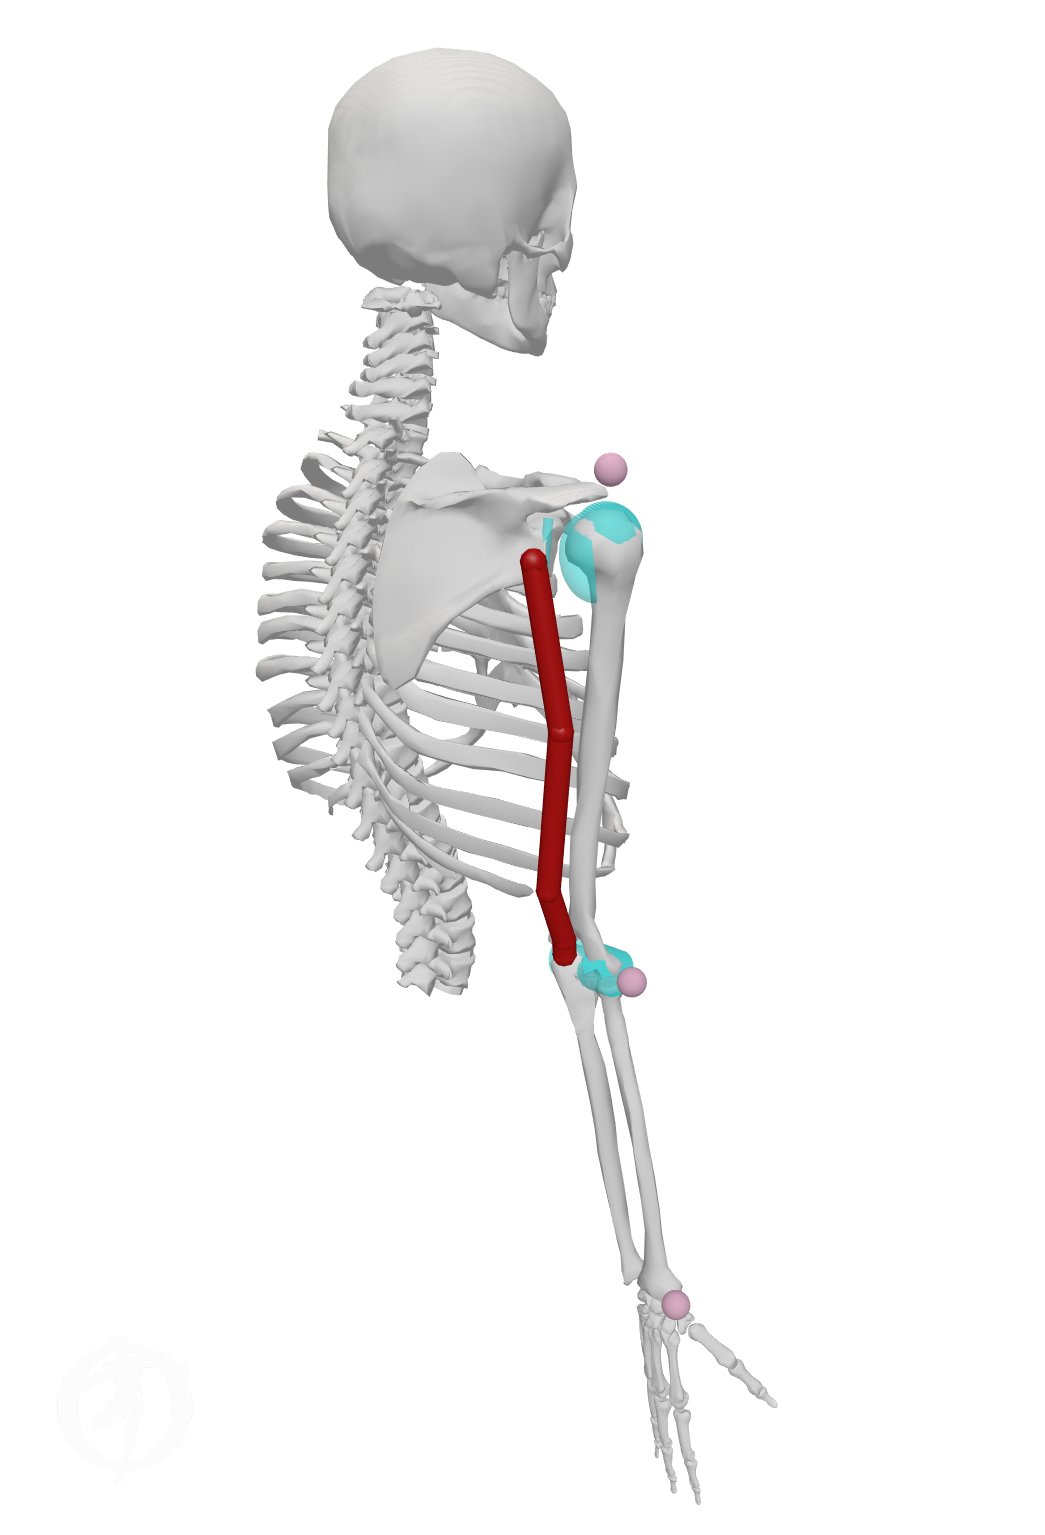
\includegraphics[width=5cm]{figure/ch4_fig_arm26Muscles_TRIlong.png}}
    \subfloat[]{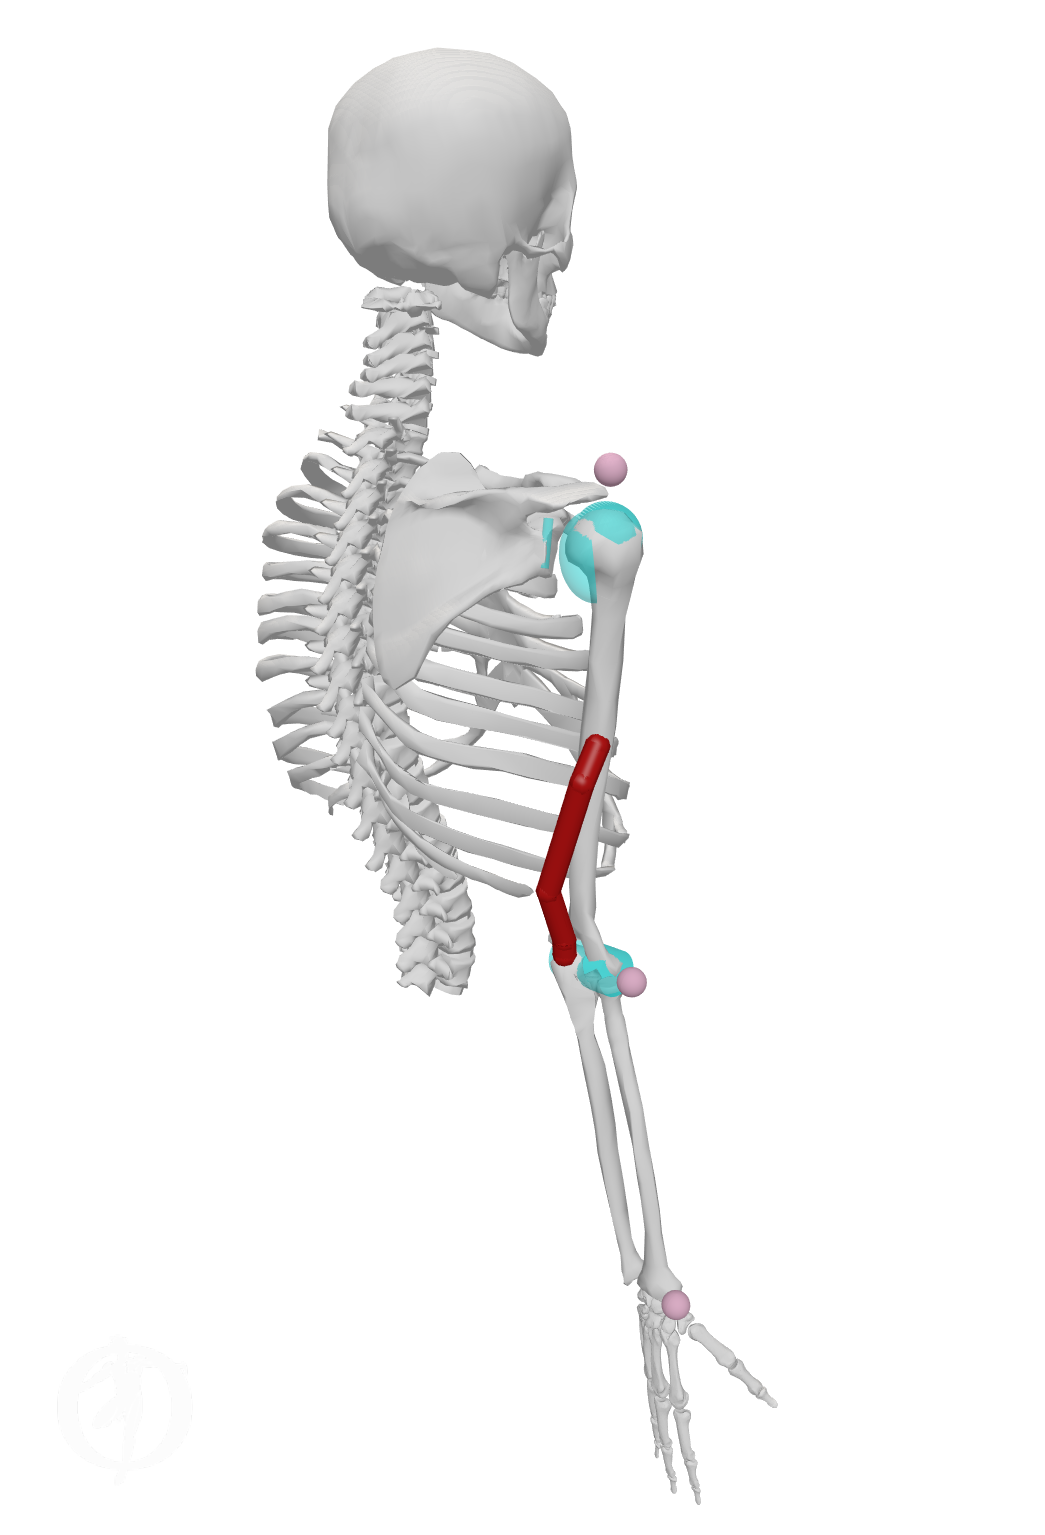
\includegraphics[width=5cm]{figure/ch4_fig_arm26Muscles_TRIlat.png}} 
    \subfloat[]{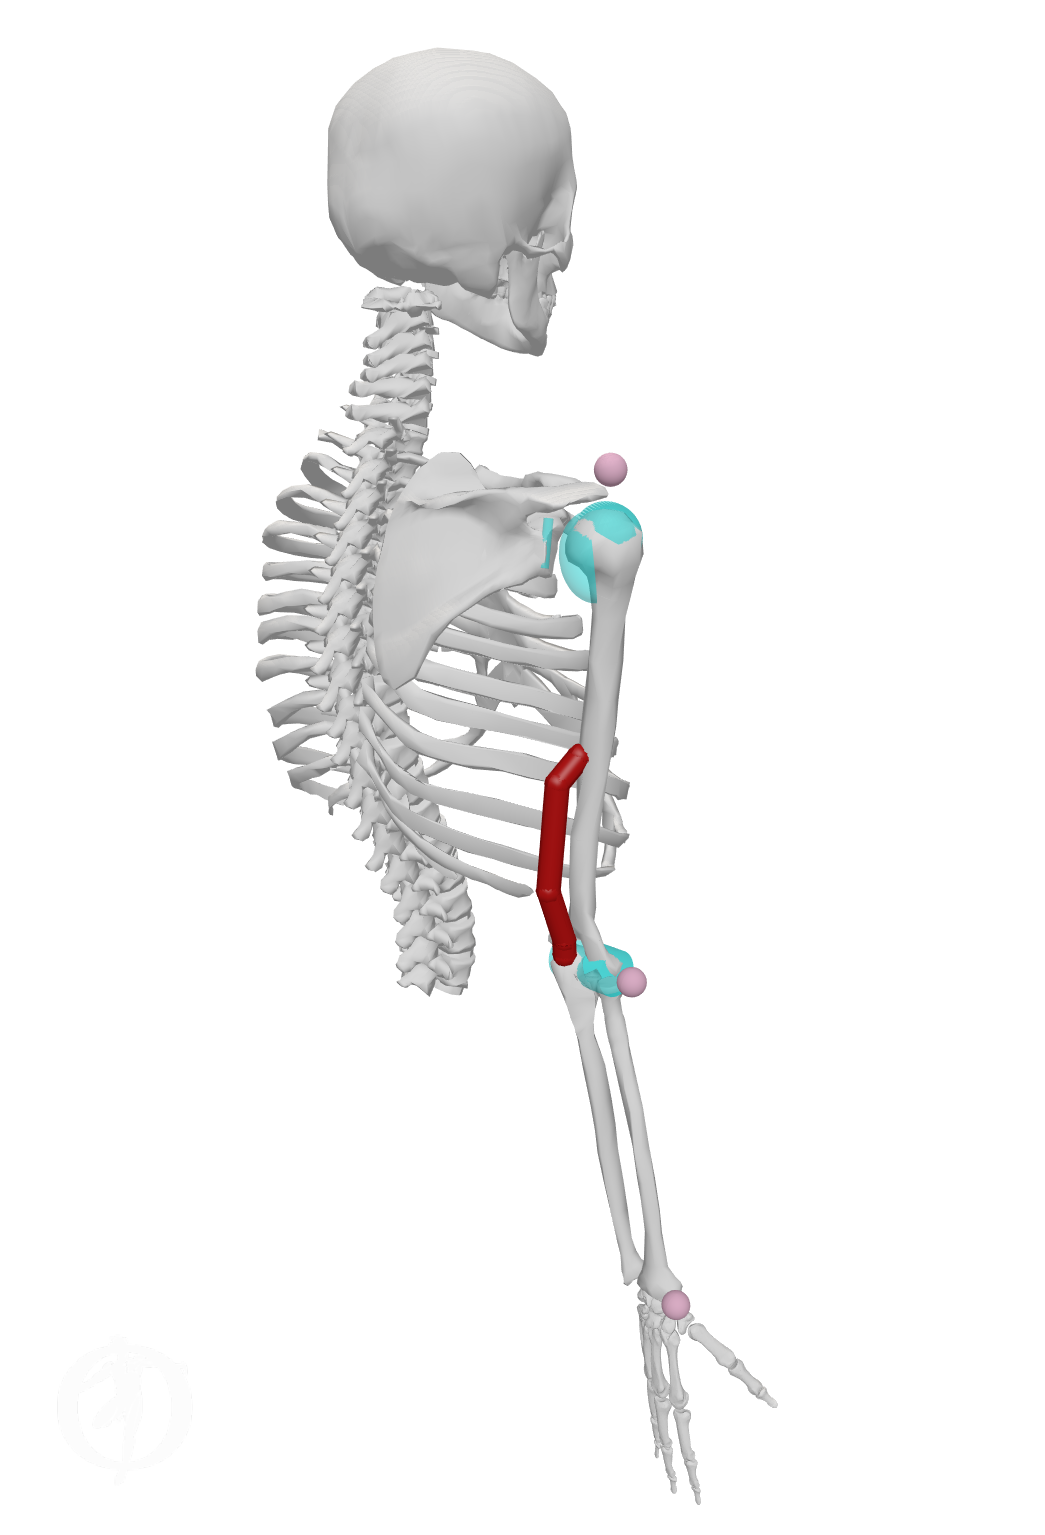
\includegraphics[width=5cm]{figure/ch4_fig_arm26Muscles_TRImed.png}} \\
    \subfloat[]{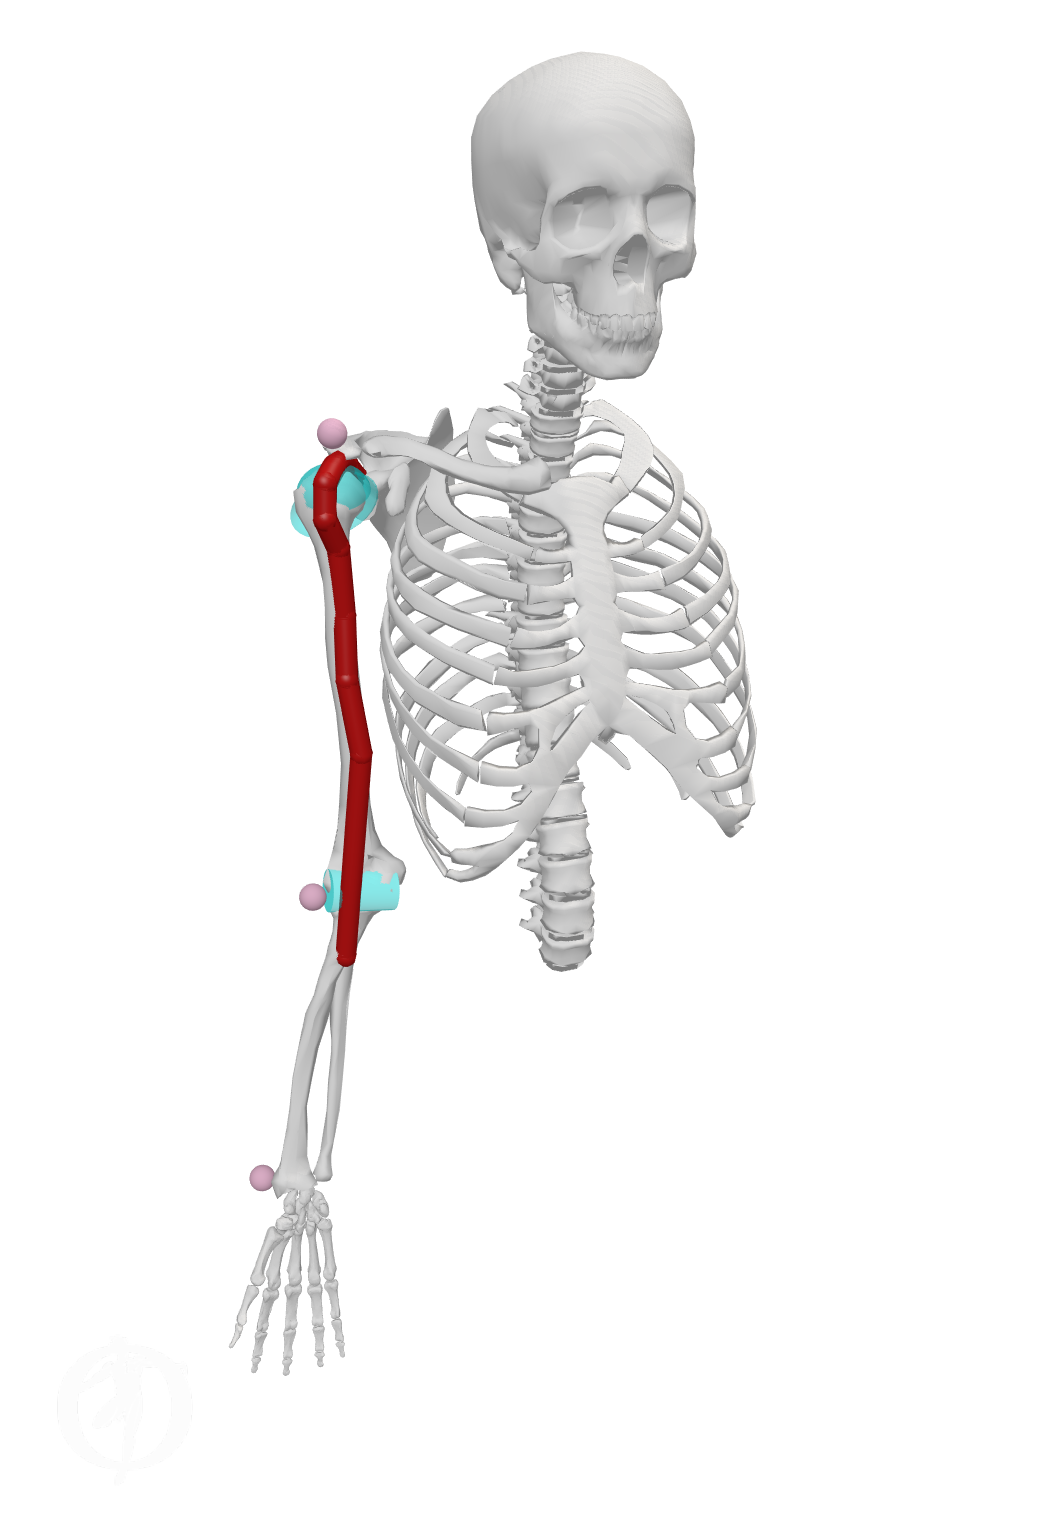
\includegraphics[width=5cm]{figure/ch4_fig_arm26Muscles_BIClong.png}}
    \subfloat[]{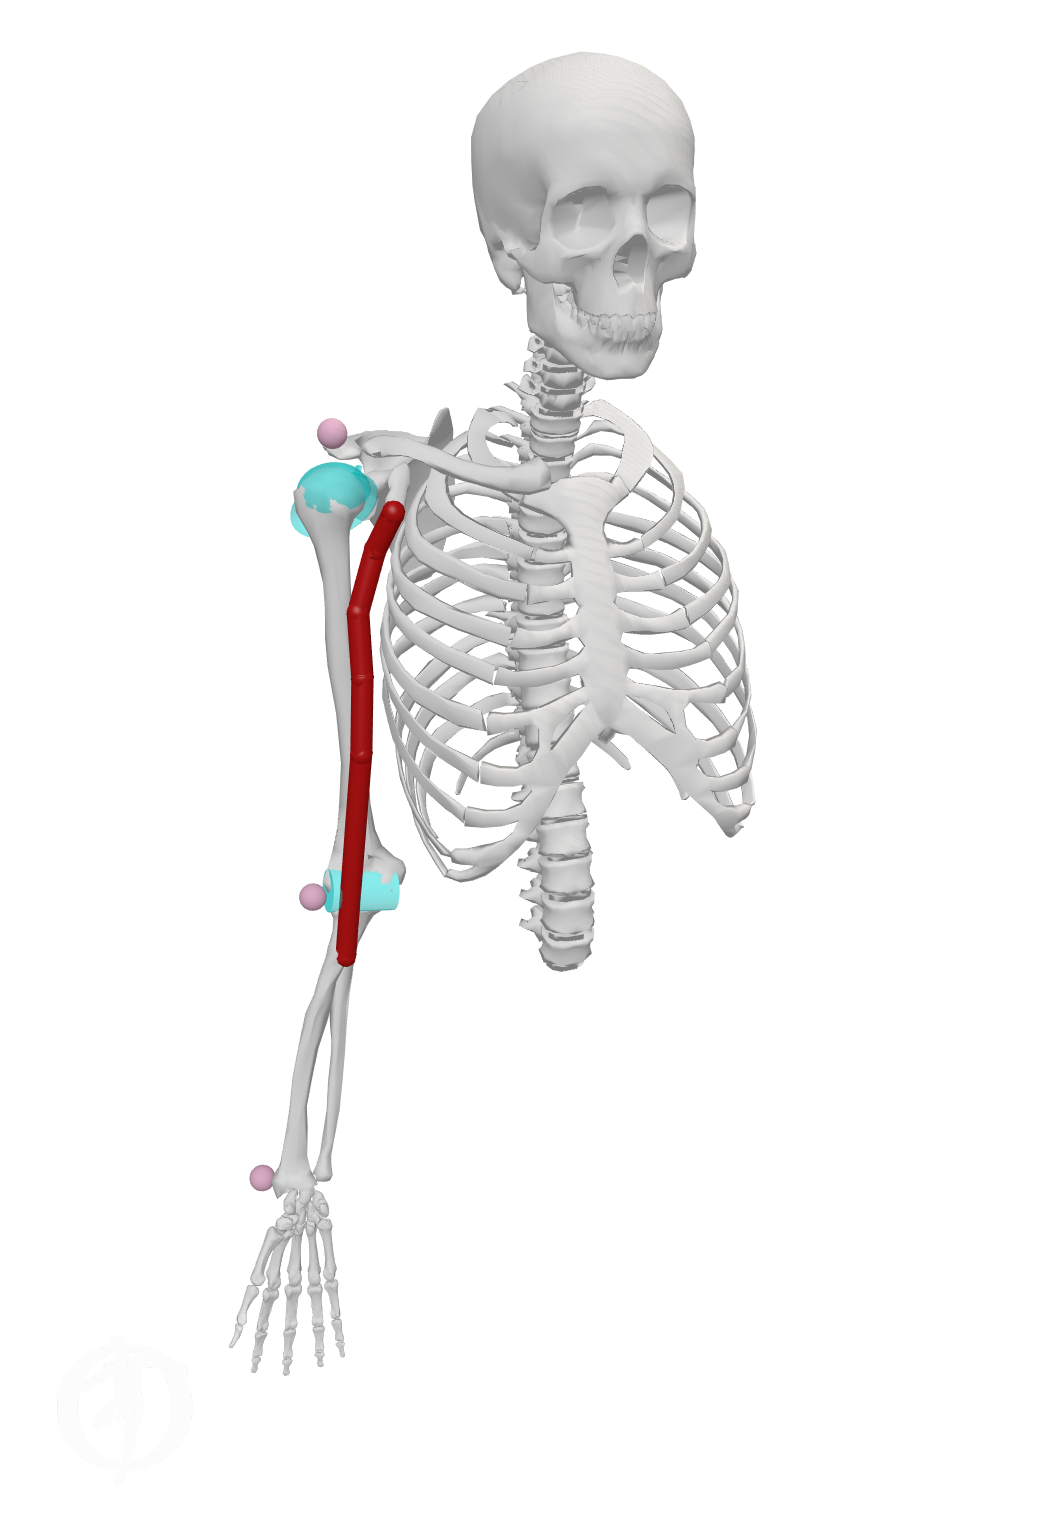
\includegraphics[width=5cm]{figure/ch4_fig_arm26Muscles_BICshort.png}}
    \subfloat[]{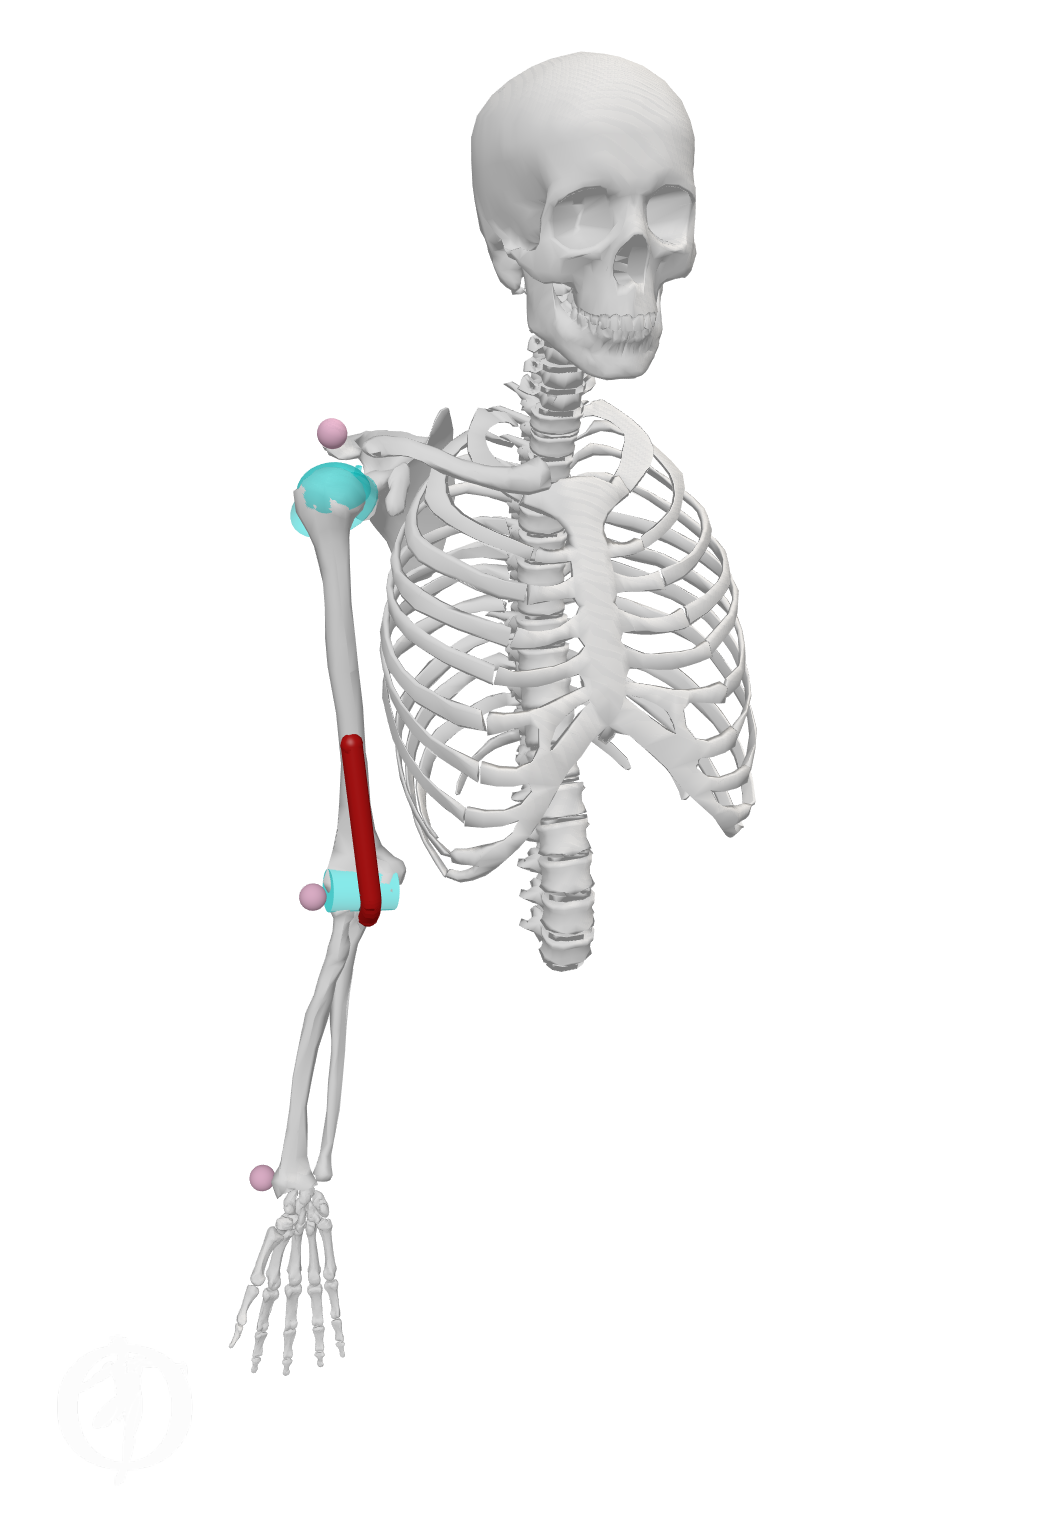
\includegraphics[width=5cm]{figure/ch4_fig_arm26Muscles_BRA.png}}
    \caption[arm26 模型之肌肉介紹]{arm26 模型所提供的六條肌肉模型,分別模擬為
                                  (a) 肱三頭肌長頭 (TRIlong)、(b) 肱三頭肌外側頭 (TRIlat)、 
                                  (c) 肱三頭肌內側頭 (TRImed)、(d) 肱二頭肌長頭 (BIClong)、
                                  (e) 肱二頭肌短頭 (BICshort) 與 (f) 肱肌 (BRA)。}
    \label{ch4_fig_arm26Muscles}
\end{figure}

\clearpage

\begin{figure}[!ht]
	\centering
	\subfloat[]{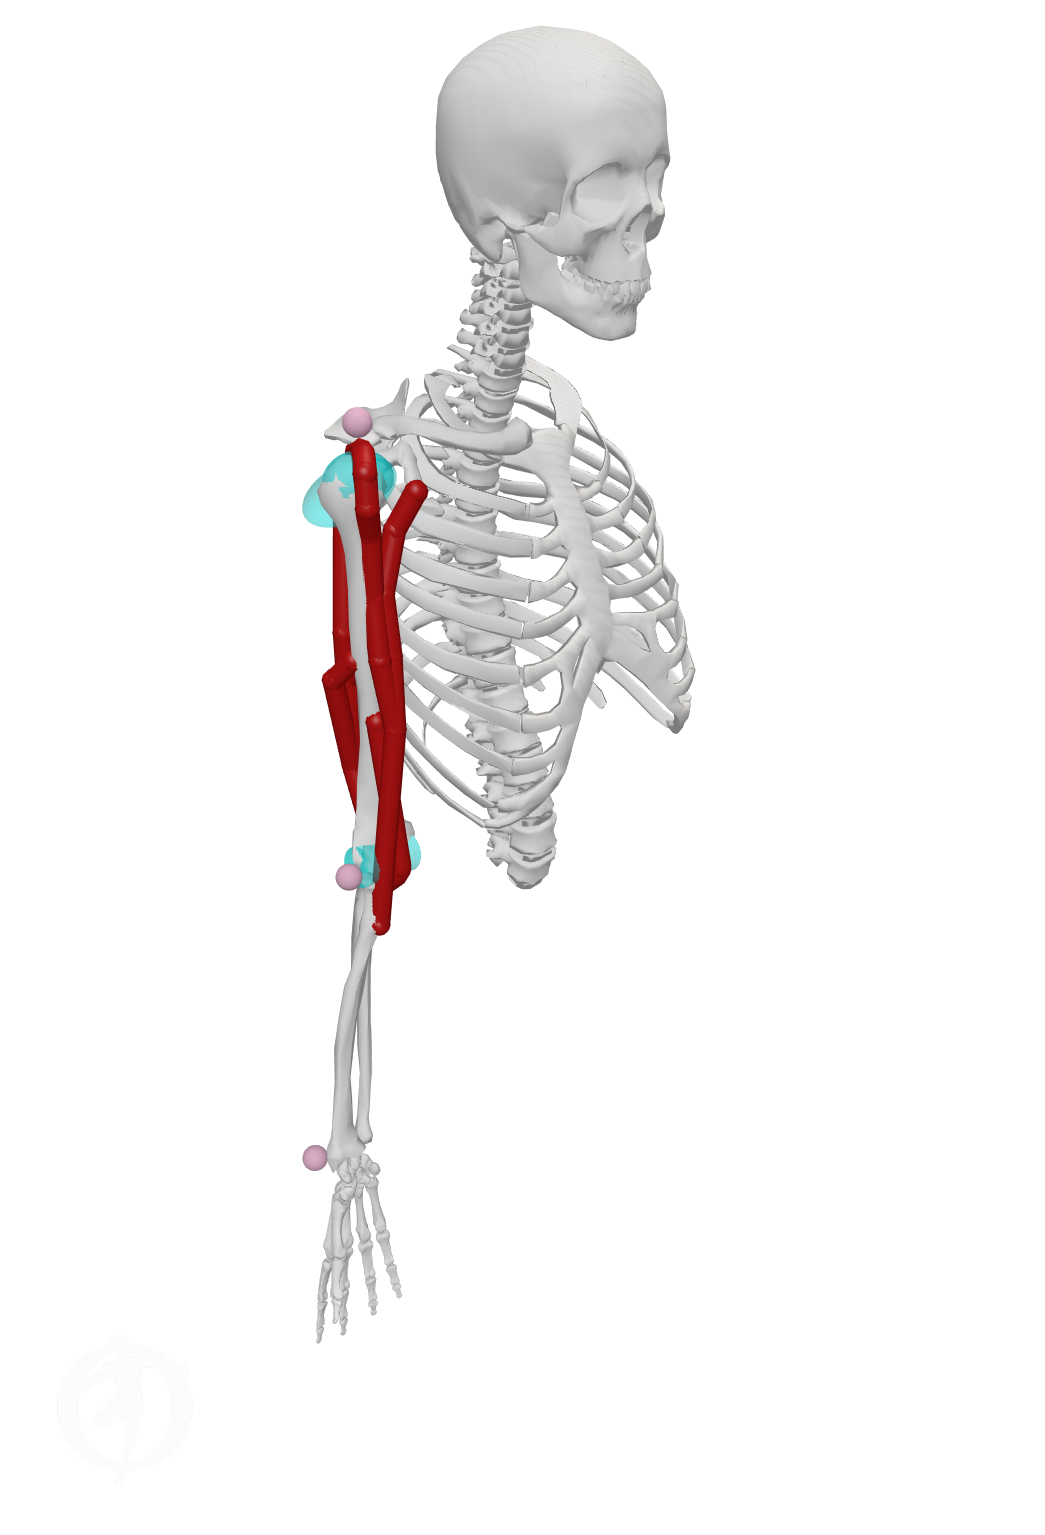
\includegraphics[width=5cm]{figure/ch4_fig_arm26Dof_0_0.png}}
    \subfloat[]{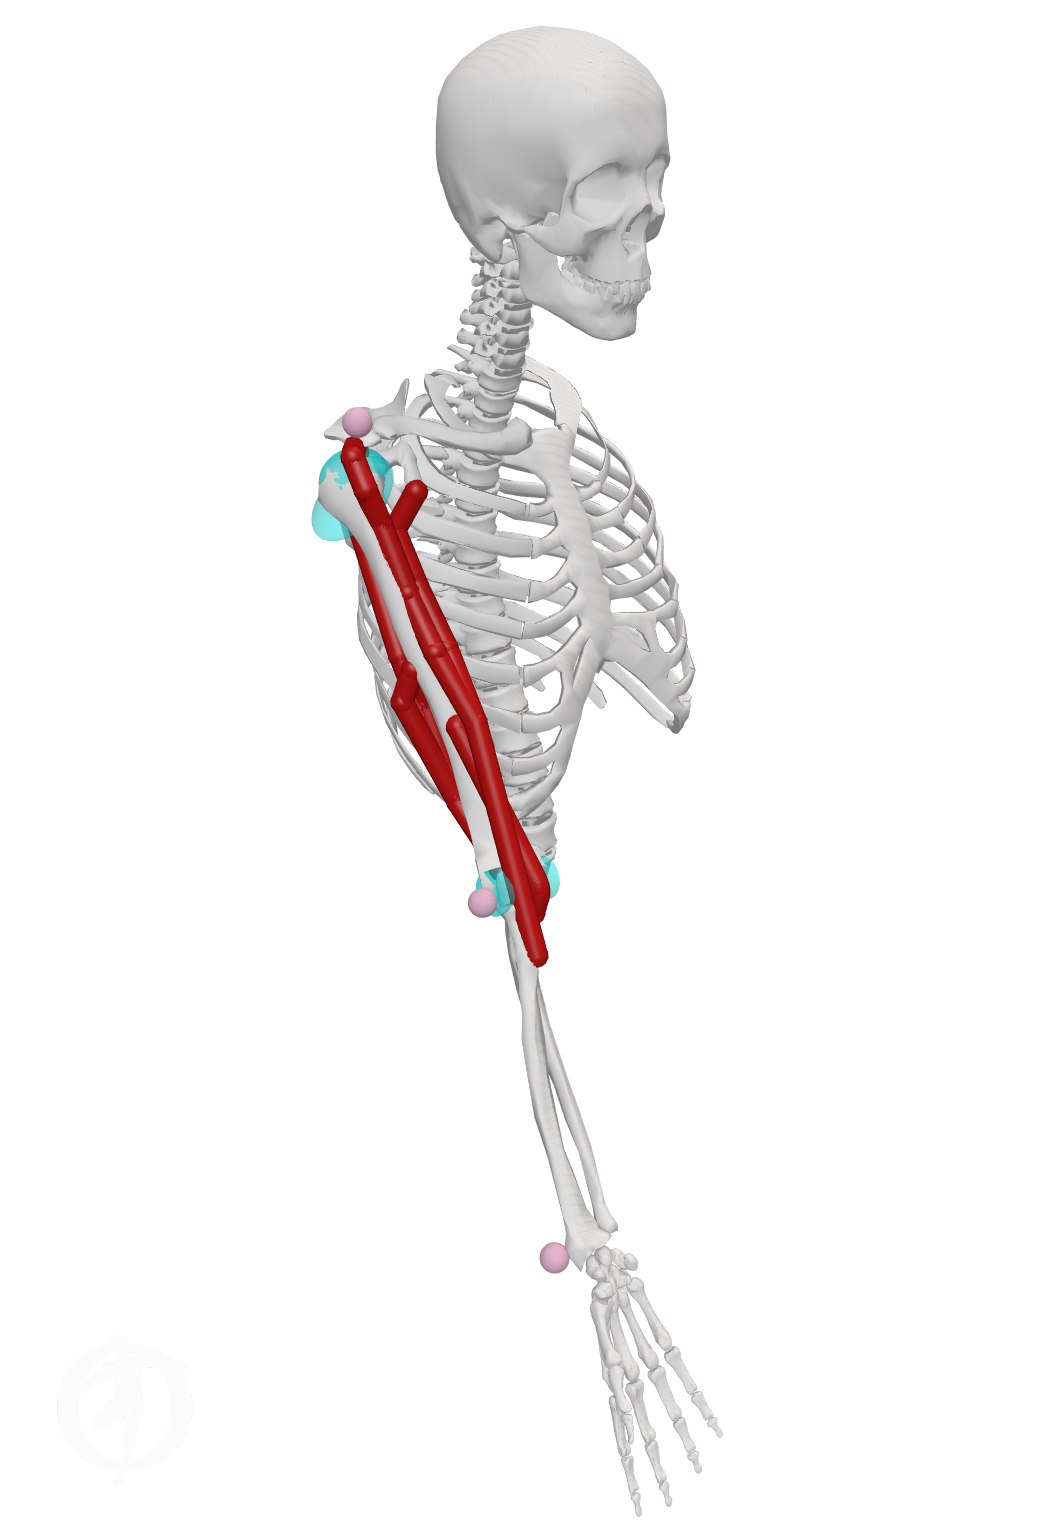
\includegraphics[width=5cm]{figure/ch4_fig_arm26Dof_30_0.png}}
    \subfloat[]{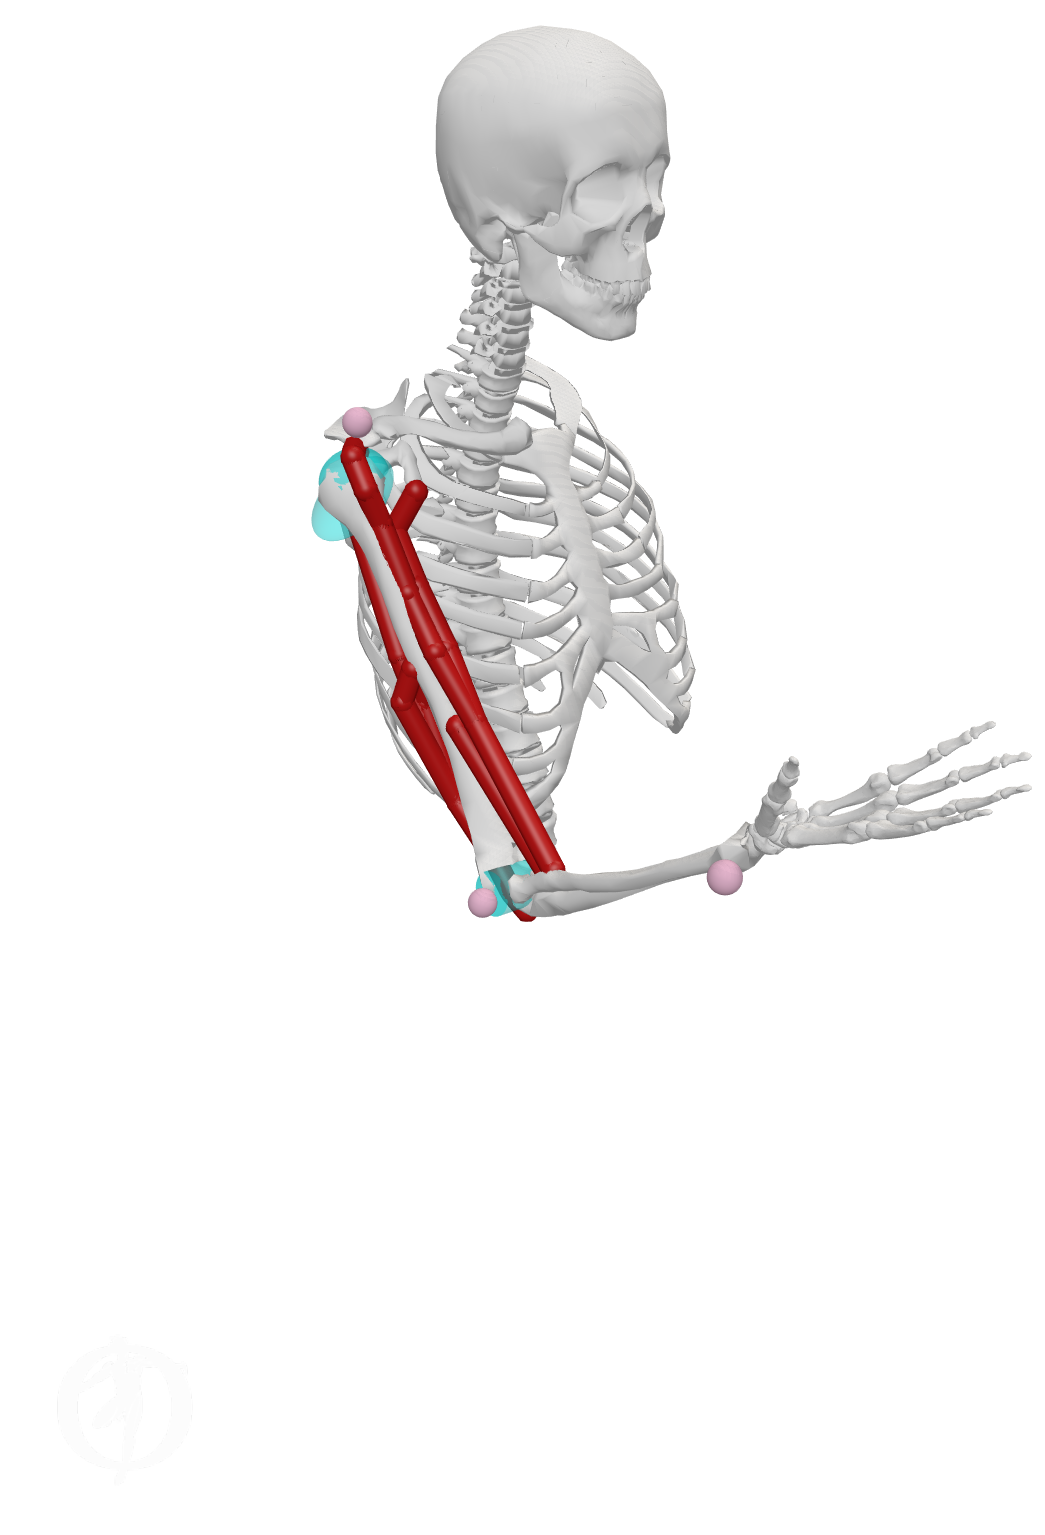
\includegraphics[width=5cm]{figure/ch4_fig_arm26Dof_30_90.png}}
    \caption[arm26 模型之自由度介紹]{arm26 模型所提供的兩個自由度,
                                    分別為肩膀或手肘的屈曲 (flexion) 和伸展 (extension),
                                    以實際移動作為展示範例:
                                    (a) $(\theta_\mathrm{shoulder}, \theta_\mathrm{elbow})=(0,0)$;
                                    (b) $(\theta_\mathrm{shoulder}, \theta_\mathrm{elbow})=(30,0)$;
                                    (c) $(\theta_\mathrm{shoulder}, \theta_\mathrm{elbow})=(30,90)$,
                                    其中單位為角度。}
    \label{ch4_fig_arm26Dof}
\end{figure}

\subsection{實驗執行}
% 負重原因;負重文獻;負重方法
本研究目的為評估肌肉參數,而適當負重使肌肉明確知道執行該動作時,需要透過哪幾條肌肉作為主動發力來抵抗負重,
故於上方介紹之 arm26 模型中,添加負重選項作為本研究之模型。負重方法參考 Akhavanfar 等學者所發表之研究,
其以抬舉任務 (lifting tasks) 作為目標動作,藉由五種不同的負重模擬方法來估計脊柱關節載荷程度,
並比較五種方法的結果差異與準確性 \cite{akhavanfar2022sharing}。
本研究採取該文獻提出之第二種方法——提高手部質量視作負重,該方法無須額外的計算分析,相較於第三種至第五種方法較為快速,
且在模擬時也同時會考慮到負重之加速度,相較於第一種方法——建立外部負載檔案,較符合真實情境。

% 負重方法;如何修改模型
本研究採取「提高手部質量」作為負重方法,但由於原先 arm26 模型之手部肢段與前臂相連,
若直接提高會代表同時提高手部與前臂的質量,模擬結果會因為慣性因素造成極大誤差,故修改原先 arm26 模型。
首先於手部位置新增一個 \ "Body" 物件,該物件質量設定為負重質量,並使用 \ "WeldJoint" 來連接手臂肢段,
讓該負重物件的移動與手臂同時進行,利用此方法來增加負重模擬,模型修正後如圖 \ref{ch4_fig_ModelwithLoad} 所示,
而該模型即為第三章所提到的標準模型或目標模型,用來作為後續的評估模型。

\clearpage

\begin{figure}[!ht]
	\centering
	\subfloat[]{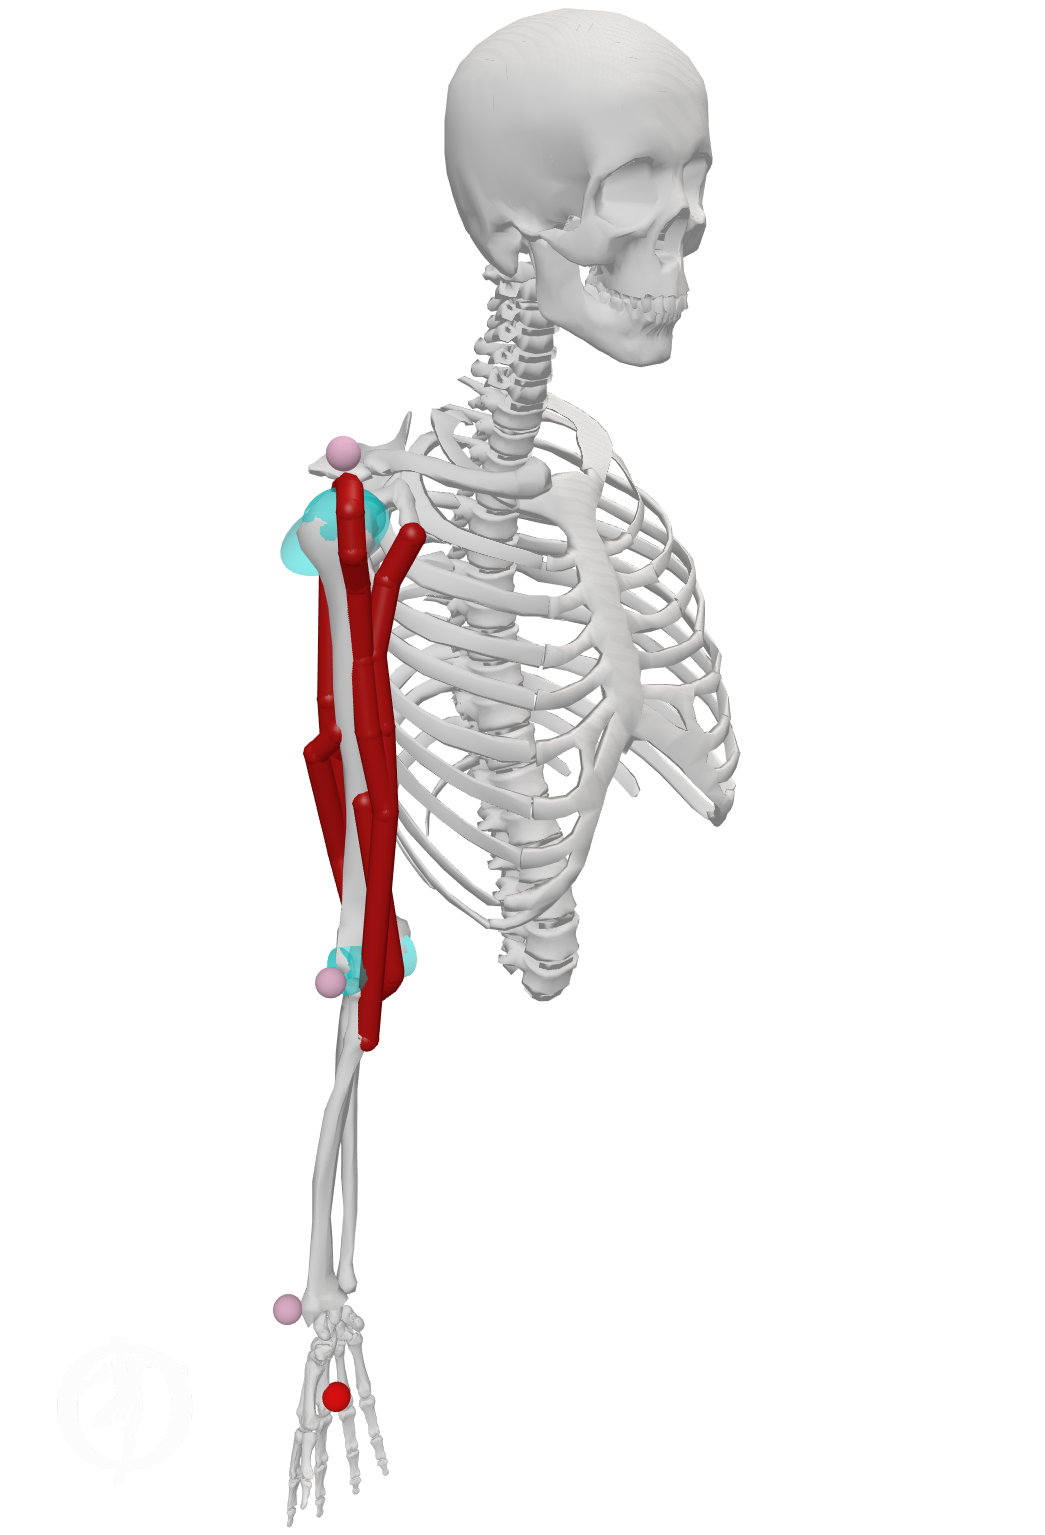
\includegraphics[width=5cm]{figure/ch4_fig_ModelwithLoad_0_0.png}}
    \subfloat[]{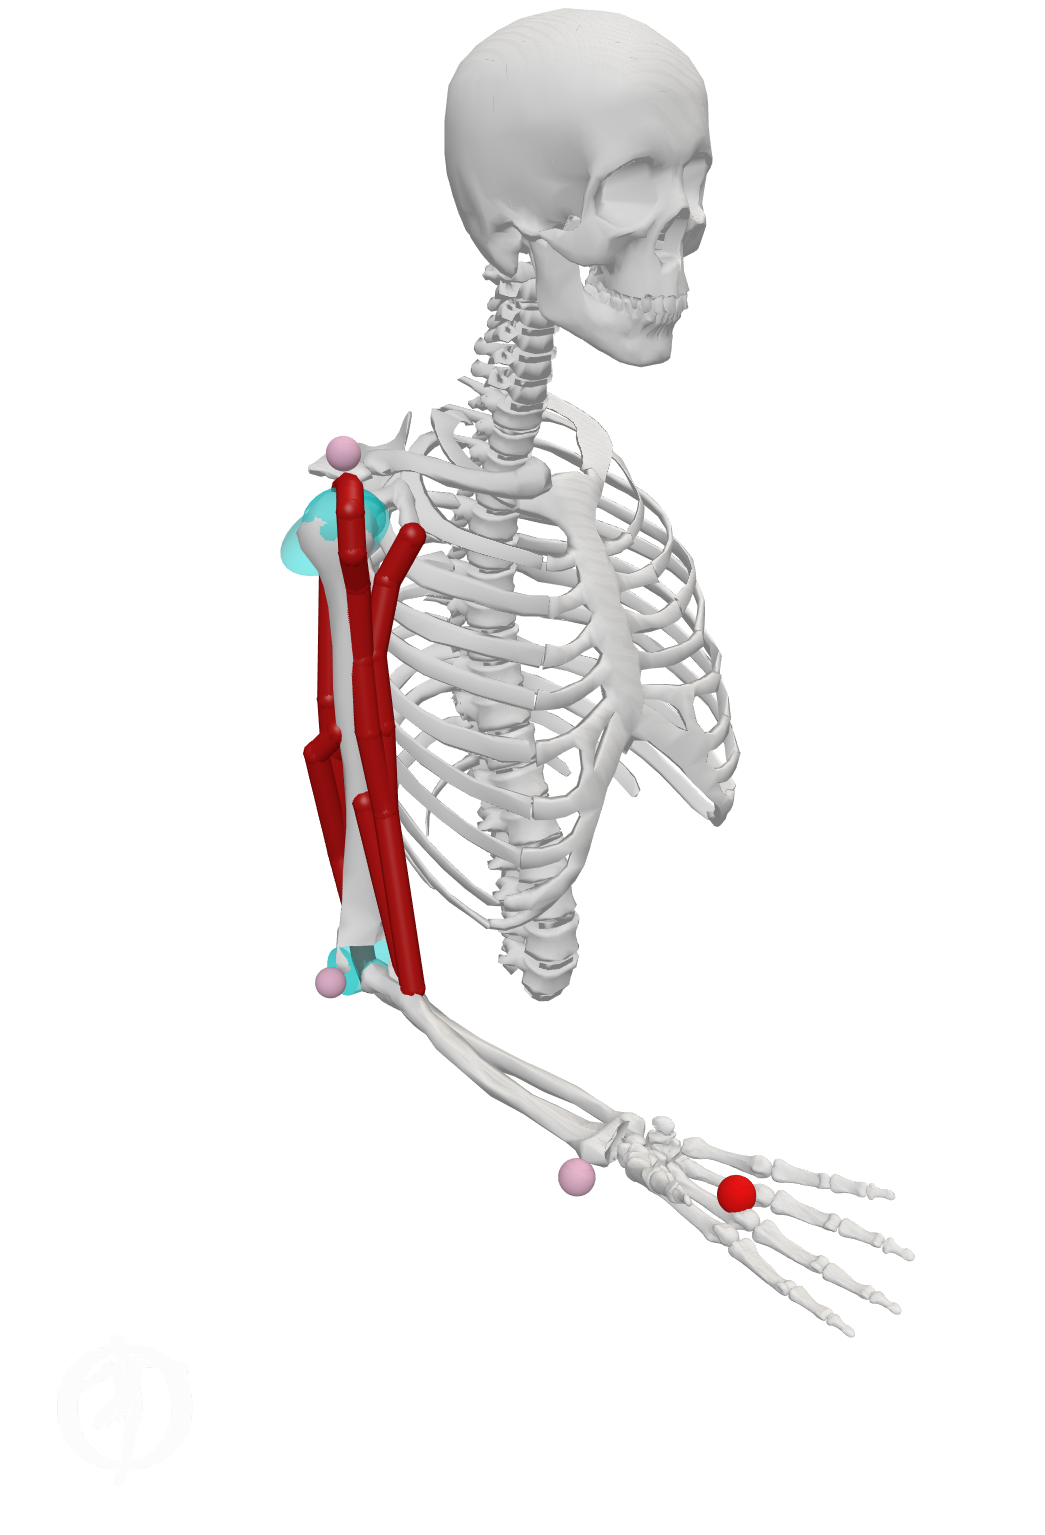
\includegraphics[width=5cm]{figure/ch4_fig_ModelwithLoad_0_90.png}}
    \caption[具負重之 arm26 模型]{具負重之 arm26 模型:
                                 (a) $(\theta_\mathrm{shoulder}, \theta_\mathrm{elbow})=(0,0)$;
                                 (b) $(\theta_\mathrm{shoulder}, \theta_\mathrm{elbow})=(0,90)$,
                                 其中單位為角度,而手部紅色圓球即為負重物件,且其與手臂同步移動。}
    \label{ch4_fig_ModelwithLoad}
\end{figure}

\subsection{誤差評估}
% 欲評估參數;預設值
本論文在模擬每條肌肉的希爾式肌肉模型當中,每條肌肉的欲評估參數之候選皆有三個,
分別為最大等長力量 ($F^\mathrm{M}_\mathrm{O}$)、最佳肌纖維長度 ($L^\mathrm{M}_\mathrm{O}$) 與
肌腱鬆弛長度($L^\mathrm{T}_\mathrm{S}$),會根據案例配置來決定最終欲評估參數之對象與數量,
無須評估之參數則設置為預設值,如下方表 \ref{ch4_table_ModelDefaultParam},
而這些預設參數值即為本論文之模擬案例的肌肉參數標準答案。

\begin{table}[!ht]
    \caption[肌肉模型預設參數]{肌肉模型預設參數}
	\label{ch4_table_ModelDefaultParam}
	\centering
    \setlength{\tabcolsep}{20pt}{
    \renewcommand\arraystretch{1.5}{ % 縱向
    \begin{tabular}{l|ccc}
        Muscle name  & $F^\mathrm{M}_\mathrm{O}$ (N) & $L^\mathrm{M}_\mathrm{O}$ (m) & $L^\mathrm{T}_\mathrm{S}$ (m) \\ \hline\hline
        TRIlong      & 798.52      & 0.1340      & 0.1430      \\ \hline
        TRIlat       & 624.30      & 0.1138      & 0.0980      \\ \hline
        TRImed       & 624.30      & 0.1138      & 0.0908      \\ \hline
        BIClong      & 624.30      & 0.1157      & 0.2723      \\ \hline
        BICshort     & 435.56      & 0.1321      & 0.1923      \\ \hline
        BRA          & 987.26      & 0.0858      & 0.0535
    \end{tabular}}}
\end{table}

\subsection{結論}

\clearpage

% ------------------------- 4.2 ------------------------- %
\section{運動軌跡與控制訊號生成}
% 生成這些要做啥?;會用到 opensim FWD 和 CMC
預測誤差作為參數估計的評斷標準,而在執行預測任務前,必須先得到指定任務的控制訊號和目標軌跡,
如同於第三章研究方法中的說明,指定任務的期望動作與實際產生的目標運動軌跡具有微小差異,
故必須先透過肌肉計算控制模擬來取得指定任務的控制訊號,再透過正向動力學模擬生成目標運動軌跡,
下方將逐一介紹本論文模擬案例的執行細節。

\subsection{期望動作生成}
% 為什麼挑這個關節;變因有哪些;單自由度簡易
本論文預測任務主要以肘關節轉動為主,根據任務的不同來決定初始角度、終止角度與轉動方向,
選擇該自由度的原因是由於欲評估之肌肉位於上臂,而肘關節的運動學正是由上臂肌肉決定,
故以肘關節轉動作為主要動作任務,另外由於肘關節為單自由度,其運動學評估簡易,適合作為研究初期之案例;
在肩關節的自由度則選擇不轉動、設定為定值,根據任務的不同來決定固定的角度。

% transformed sine motion;time dutation;time shift
本研究將肘關節的轉動軌跡擬合為正弦函數,根據振幅、週期、平移的調配,來生成符合轉動的方程式,
其中方程式又區分成屈曲與伸展兩種,屈曲軌跡生成為公式 \ref{ch4_eqn_TrajFlex},而伸展則為公式 \ref{ch4_eqn_TrajExten}:
\begin{equation}
    \mathit{Tr}_\mathrm{F}(t) =
    \begin{cases}
        \theta_1 & \text{when} \quad t \leq T \\
        \frac{\theta_2 - \theta_1}{2} \sin[\frac{2 \ \pi}{2 \ t_\mathrm{dur}} (t-T) - \frac{\pi}{2}]
         + \frac{\theta_2 - \theta_1}{2} + \theta_1 & \text{when} \quad T < t \leq T + t_\mathrm{dur} \\
        \theta_2 & \text{when} \quad t > T + t_\mathrm{dur}
    \end{cases}
    \label{ch4_eqn_TrajFlex}
\end{equation}
\begin{equation}
    \mathit{Tr}_\mathrm{E}(t) =
    \begin{cases}
        \theta_2  & \text{when} \quad t \leq T \\
        \frac{\theta_2 - \theta_1}{2} \sin[\frac{2 \ \pi}{2 \ t_\mathrm{dur}} (t-T) + \frac{\pi}{2}]
         + \frac{\theta_2 - \theta_1}{2} + \theta_1 & \text{when} \quad T < t \leq T + t_\mathrm{dur} \\
        \theta_1  & \text{when} \quad t > T + t_\mathrm{dur}
    \end{cases}
    \label{ch4_eqn_TrajExten}
\end{equation}
其中軌跡函式 $\mathit{Tr}$ 主要由轉動角度波谷值 $\theta_1$ 與波峰值 $\theta_2$ 決定,若為屈曲運動,
則 $\theta_1$ 為初始角度、$\theta_2$ 為終止角度,反之若為伸展運動,則 $\theta_2$ 為初始角度、
$\theta_1$ 為終止角度,故 $\theta_2$ 必定大於 $\theta_1$;
轉動所需要的時間 $t_\mathrm{dur}$ 則根據轉動範圍來換算,以轉動 130 度需要 1 秒的比例進行縮放,換算公式為
$t_\mathrm{dur} = \frac{\theta_2 - \theta_1}{130}$;時間平移 $T$ 則設定為 0.03 秒定值,
故轉動會在 0.03 秒後才開始執行,目的是為了配合 OpenSim 肌肉計算控制模擬需要 0.03 秒的緩衝時間,
下方圖 \ref{ch4_fig_DesiredTrajExample} 為期望動作的生成範例。

\clearpage

\begin{figure}[!ht]
	\centering
	\subfloat[]{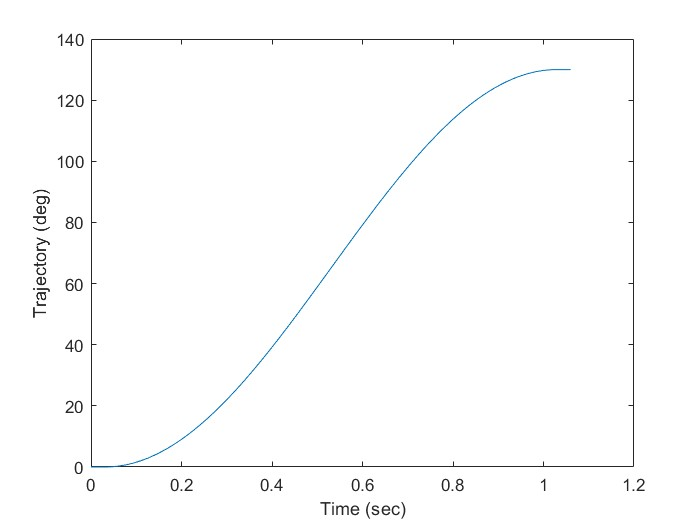
\includegraphics[width=7cm]{figure/ch4_fig_DesiredTrajExample_F_0_0_130.jpg}}
    \subfloat[]{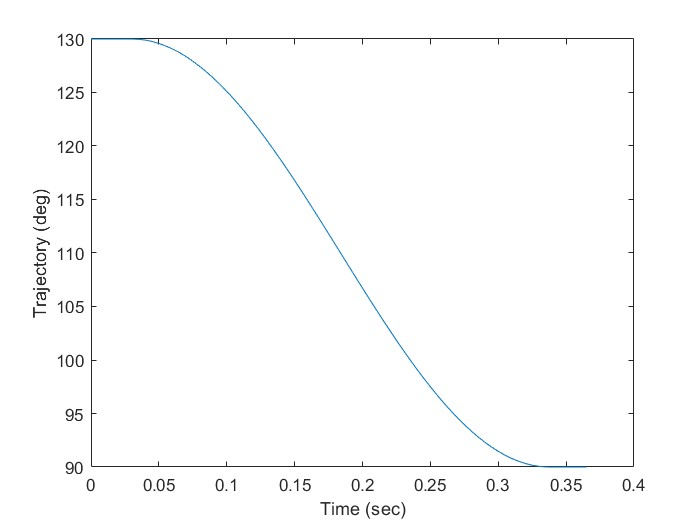
\includegraphics[width=7cm]{figure/ch4_fig_DesiredTrajExample_E_180_90_130.jpg}}
    \caption[期望動作生成範例]{期望動作被擬合為正弦函數,其根據公式 \ref{ch4_eqn_TrajFlex} 與 \ref{ch4_eqn_TrajExten} 生成:
                             (a) 執行屈曲動作,參數配置為 $(\theta_1, \theta_2)=(0,130)$,
                             由轉動範圍縮放得到 $t_\mathrm{dur} = 1 $ 秒;
                             (b) 執行伸展動作,參數配置為 $(\theta_1, \theta_2)=(90,130)$,
                             由轉動範圍縮放得到 $t_\mathrm{dur} = 0.3077 $ 秒。}
    \label{ch4_fig_DesiredTrajExample}
\end{figure}

\subsection{控制訊號生成}
% 步驟;XML 檔設定;output 會是 XML control 檔案
取得期望動作後,將該動作資料與目標模型輸入至肌肉計算控制模擬中,來取得目標模型生成該期望動作所需的控制訊號。
在肌肉計算控制模擬設置中,如圖 \ref{ch3_flowchart_CMC} 所示,還需 \ "Tracking\_Task"、
"Reserve\_Actuators" 與 \ "Control\_Constraints" 三個檔案輸入至 \ "CMC\_Setup" 中,
這些檔案以原先 OpenSim 於 Arm26 資料夾內所提供的檔案進行設置,但在 \ "Control\_Constraints" 檔案中,
每條肌肉的 \ "default\_min" 皆調整為 0.001。經過肌肉計算控制模擬後,將會得到控制訊號、模型狀態等資訊,
將於下階段模擬使用。

\subsection{運動軌跡生成}
% FWD 運動軌跡;FWD XML
以肌肉計算控制得到的控制訊號作為輸入,模型狀態作為初始狀態,輸入目標模型至正向動力學模擬,
即可得到最終的目標運動軌跡,該軌跡為目標模型能達成最相似期望動作的軌跡,且包含肌肉於各時間點的狀態、力量等資訊,
若當輸入不同的模型至模擬時,將會產生不同的運動軌跡,如預測模型、擾動模型等皆會有相異結果,這些軌跡將與目標軌跡比較,
作為後續敏感度分析、多運動軌跡預測最佳化、驗證模型的評估標準。在正向動力學模擬設置中,由於有提供初始狀態,
故設定 \ "solve\_for\_equilibrium\_for\_auxiliary\_states" 為 \ "false",
並提供相同的 \ "Reserve\_Actuators" 檔案,其餘則設定為預設。

\clearpage

% error 情形發生說明;nan
在 OpenSim 的正向動力學文檔 \cite{opensim_fwd} 中表明,由於是透過積分器運算,且為開迴路系統,
故在積分過程可能會因為數值誤差的累積,造成結果隨時間漂移,另外若當問題太過僵硬,
可能會造成積分器需要極小的時間步長,該情況會讓模擬執行緩慢並生成大量的結果。
本研究在後續執行過程皆有遇到相似的問題,是由於肌肉參數在擾動或尋找過程中,可能會產生不合常理的參數組合,
故若發生相似的問題時,本研究將該些情況的誤差直接設置為 \ "nan",不予以處理與考量。
% 而若模擬超過一定時長,也將強制終止並同樣設置誤差為  \ "nan"。

% ------------------------- 4.3 ------------------------- %
\section{任務與肌肉參數間之敏感度分析}
% 敏感度分析概念和目的
從預測任務中來評估參數為本研究核心概念,「任務」的組成由負重和動作兩者共同決定,
透過設定先前介紹的具負重之上肢肌肉骨骼模型,來選擇手部負重質量,而動作如同先前介紹之期望動作生成,
可根據肘關節的轉動角度與方向、肩關節的固定角度來決定,不同的任務組合都會對每條肌肉產生相異的敏感度指標。
本節將透過全因子的實驗設計法,計算所分類出的全部任務之敏感度指標,從該分析結果來挑選合適的任務,
作為後續最佳化與驗證模型的執行任務。

\subsection{任務種類}
% load; direction; shoulder angle; elbow angle
\begin{table}[!b]
    \caption[任務種類編號範例]{任務種類編號範例}
	\label{ch4_table_TaskIndex}
	\centering
    \setlength{\tabcolsep}{16pt}{
    \renewcommand\arraystretch{1.5}{ % 縱向
    \begin{tabular}{l|ccc}
        任務編號    & $V_\mathrm{dir}$  & $\theta_\mathrm{sh}$ (deg) & $[\theta_1,\theta_2]$ (deg) \\ \hline\hline
        Task 1     & flexion   & -90    & [0,90]     \\
        Task 2     & flexion   & -90    & [0,130]    \\
        Task 3     & flexion   & -90    & [90,130]   \\
        Task 4     & flexion   & -45    & [0,90]     \\
        \multicolumn{1}{c|}{$\vdots $}  & \multicolumn{3}{c}{$\vdots $} \\
        Task 21    & flexion   & 180    & [90,130]   \\
        Task 22    & extension & -90    & [0,90]     \\
        \multicolumn{1}{c|}{$\vdots $}  & \multicolumn{3}{c}{$\vdots $} \\
        Task 42    & extension & 180    & [90,130]   \\
    \end{tabular}}}
\end{table}

為了簡化模擬複雜度,模擬案例中的模型負重皆設定為 2.5 公斤,不予以更動,而在動作任務分類上共含有三個因子,
分別為肘關節轉動方向 $V_\mathrm{dir}$、肩關節角度 $\theta_\mathrm{sh}$,以及肘關節角度組合 $[\theta_1,\theta_2]$。
肘關節轉動方向因子含有 2 個水準,分別為 $V_\mathrm{dir} = \{\text{flexion}, \text{extension}\}$;
肩關節角度因子含有 7 個水準,分別為 $\theta_\mathrm{sh} = \{-90,-45,0,45,90,135,180\}$,單位為角度;
肘關節角度組合因子含有 3 個水準,分別為 $[\theta_1, \theta_2] = \{[0,90],[0,130],[90,130]\}$,單位為角度。
最終組合成的任務共含有 42 種供挑選,並依照上方說明順序進行編號,上方表 \ref{ch4_table_TaskIndex} 為編號範例,
其餘任務編號將以此類推,其中肘關節轉動方向 $V_\mathrm{dir}$ 與肘關節角度組合 $[\theta_1,\theta_2]$ 用於公式 \ref{ch4_eqn_TrajFlex} 和 \ref{ch4_eqn_TrajExten} 之期望動作生成,
而肘關節與肩關節角度所對應之模型姿態可參考圖 \ref{ch4_fig_arm26Dof} 和 \ref{ch4_fig_ModelwithLoad}。

\subsection{任務挑選準則}
% 最佳化任務挑選;常見訓練動作;為何不是挑敏感度高的
在任務挑選準則上,將其分成供「最佳化階段」與供「模型驗證階段」使用來討論,
最佳化任務的挑選將以常見的健身動作作為執行任務,例如以啞鈴彎舉來評估二頭肌參數,
而先前增加的負重功能即可作為啞鈴重量來源的模擬,此階段的敏感度分析則用來檢測該動作是否可行。
之所以不挑選敏感度最高的動作是由於最佳化演算法所故,本研究在最佳化過程所設定的上下界較為寬鬆,
第一階段的最佳化過程 (尋找初始值) 大多在距離最佳參數甚遠的地方進行迭代,
而敏感度分析只代表在預設參數擾動範圍內的敏感度 (如 $\pm 5\%$),
故兩個不同範圍的評估結果是沒有相關聯的 (最佳化範圍指的是上下界,敏感度分析指的則是擾動範圍),
若選擇高敏感度任務給最佳化執行,則可能會造成很難、甚至無法收斂,使得參數評估時間增長或失敗,
不過若當最佳化的上下界與敏感度分析的擾動範圍相同,例如皆為最佳參數的 $\pm 5\%$,
則應挑選高敏感度任務來進行最佳化參數評估,但該情形於本研究並不探討。

% 模型驗證任務挑選;為何是挑敏感度高的
模型驗證階段則與敏感度分析結果相關,模型驗證的目的是為了確保最佳模型在執行其他任務時仍有低誤差的表現,
此時最佳模型裡的參數有兩種可能,第一種為與預設答案相近,若設定敏感度分析的擾動值為 $\pm 5\%$ 或更小,
則兩者 (模型驗證與敏感度分析) 是相關聯的,故應挑選高敏感度任務來驗證;第二種則為與預設答案相差甚遠的參數結果,
但由於預測誤差小到使得最佳化中斷,此種情形涉及到參數不可識別性,將在後續案例會深入探討,不過該狀況在執行其他任務時,
皆會有巨大的預測誤差,因此同樣挑選高敏感度的任務即可。綜合上述,在模型驗證的任務挑選準則上,
將優先挑選高敏感度的任務來執行,但若任務在 NRMSE 為 nan 之樣本數量過多,則不予以考量。

\clearpage

\subsection{敏感度分析}
% 執行次數;全因子的實驗設計法 (full factorial design);程式流程圖
如同於第三章所述,若模型含有 $N_\mathrm{m}$ 條肌肉和 $N_\mathrm{k}$ 個任務需要評估,
則需執行 $N_\mathrm{m} \times N_\mathrm{k}$ 次敏感度分析,本模擬案例的模型雖含有 6 條肌肉,
但欲評估之肌肉只有二頭肌群的 2 條肌肉,在全因子的實驗設計下共有 42 個任務需要評估,
故需執行 $2 \times 42 = 84$ 次敏感度分析,每次的敏感度分析皆會得到一個對應指標,
其用來代表該肌肉與該任務的關聯性,指標大意味著該肌肉在相同範圍的擾動下,執行該任務時會有更大的運動軌跡偏移,
而這些敏感度分析結果可用來檢測和挑選最佳化與驗證模型階段的執行任務,其程式執行流程圖如圖 \ref{ch4_flowchart_SA} 所示。

\bigskip
\begin{figure}[!ht]
	\centering
	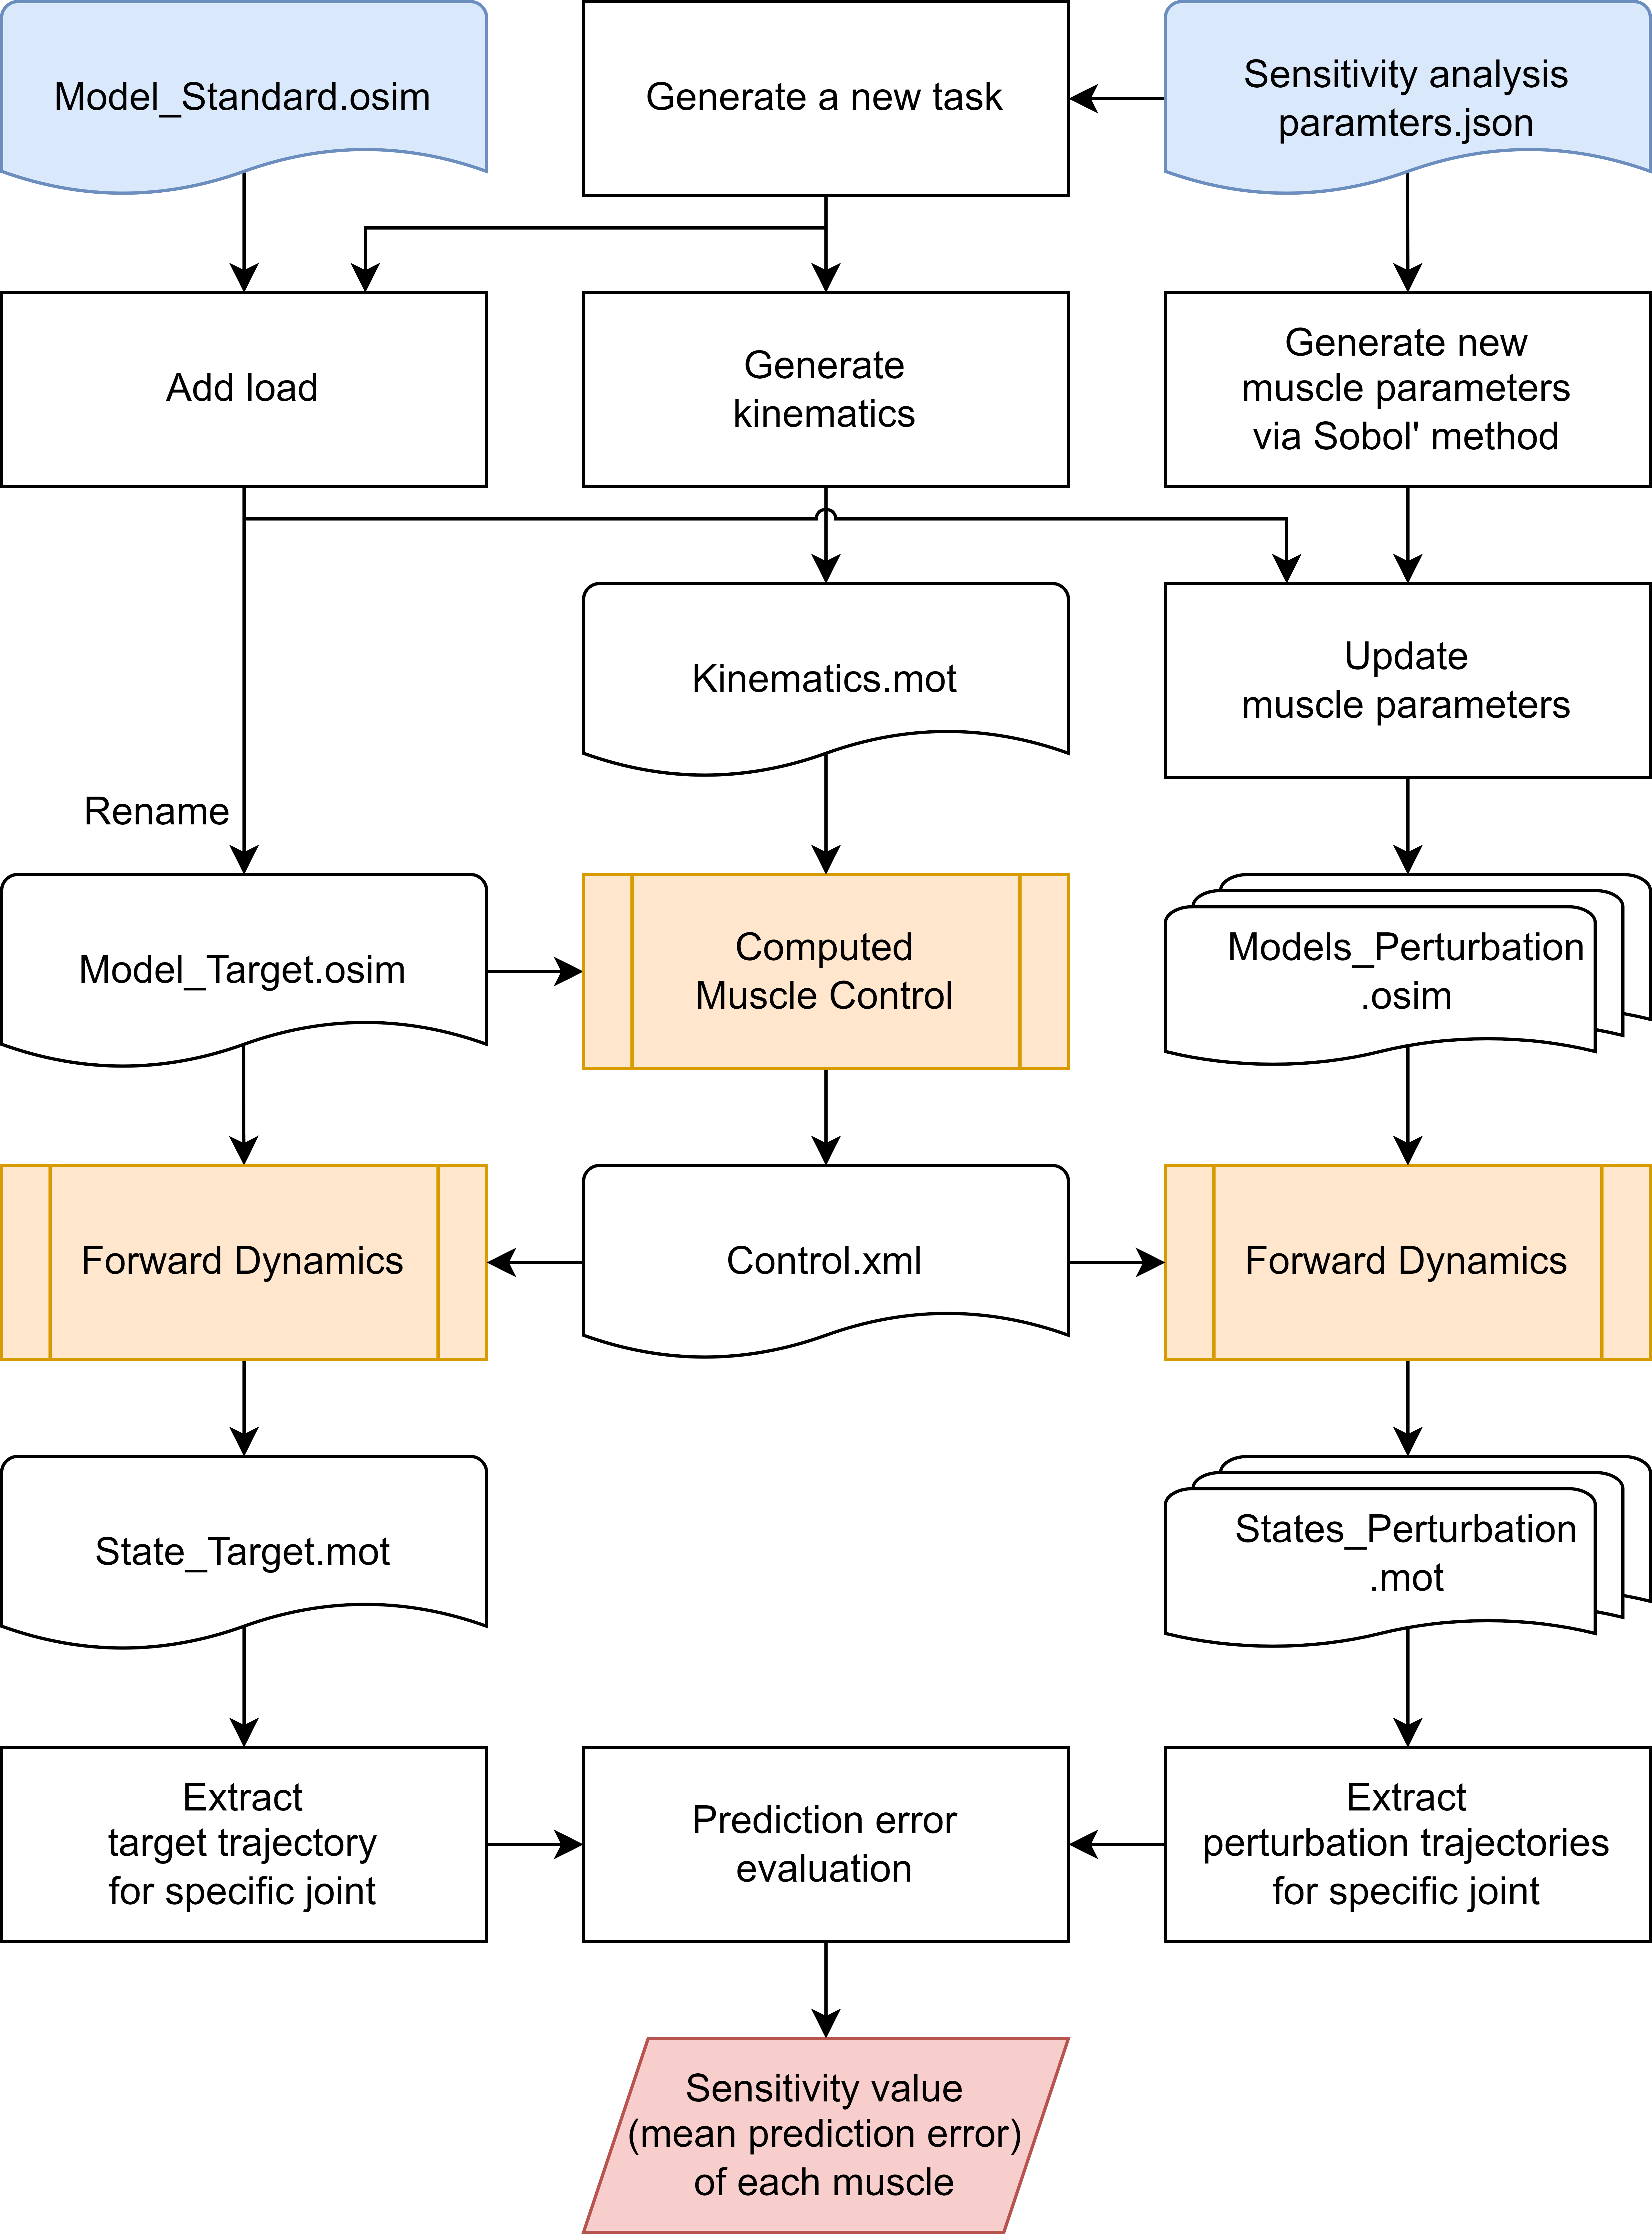
\includegraphics[width=11.5cm]{figure/ch4_flowchart_SA.PNG}
    \caption[敏感度分析之程式執行流程圖]{敏感度分析之程式執行流程圖}
    \label{ch4_flowchart_SA}
\end{figure}

\clearpage

% 參數設定和代表意義;執行結果
在本模擬案例中,敏感度分析的參數設定為樣本 $N_\mathrm{sa} = 500$ 與擾動值 $\delta = 0.05$,
代表透過 Sobol 序列來生成 500 個隨機參數組合,且均落在欲評估肌肉預設值的 $\pm 5\%$ 之內,
下方圖 \ref{ch4_fig_SAResults} 為二頭肌長頭與短頭對各任務之敏感度指標。

\bigskip
\begin{figure}[!ht]
	\centering
	\subfloat[]{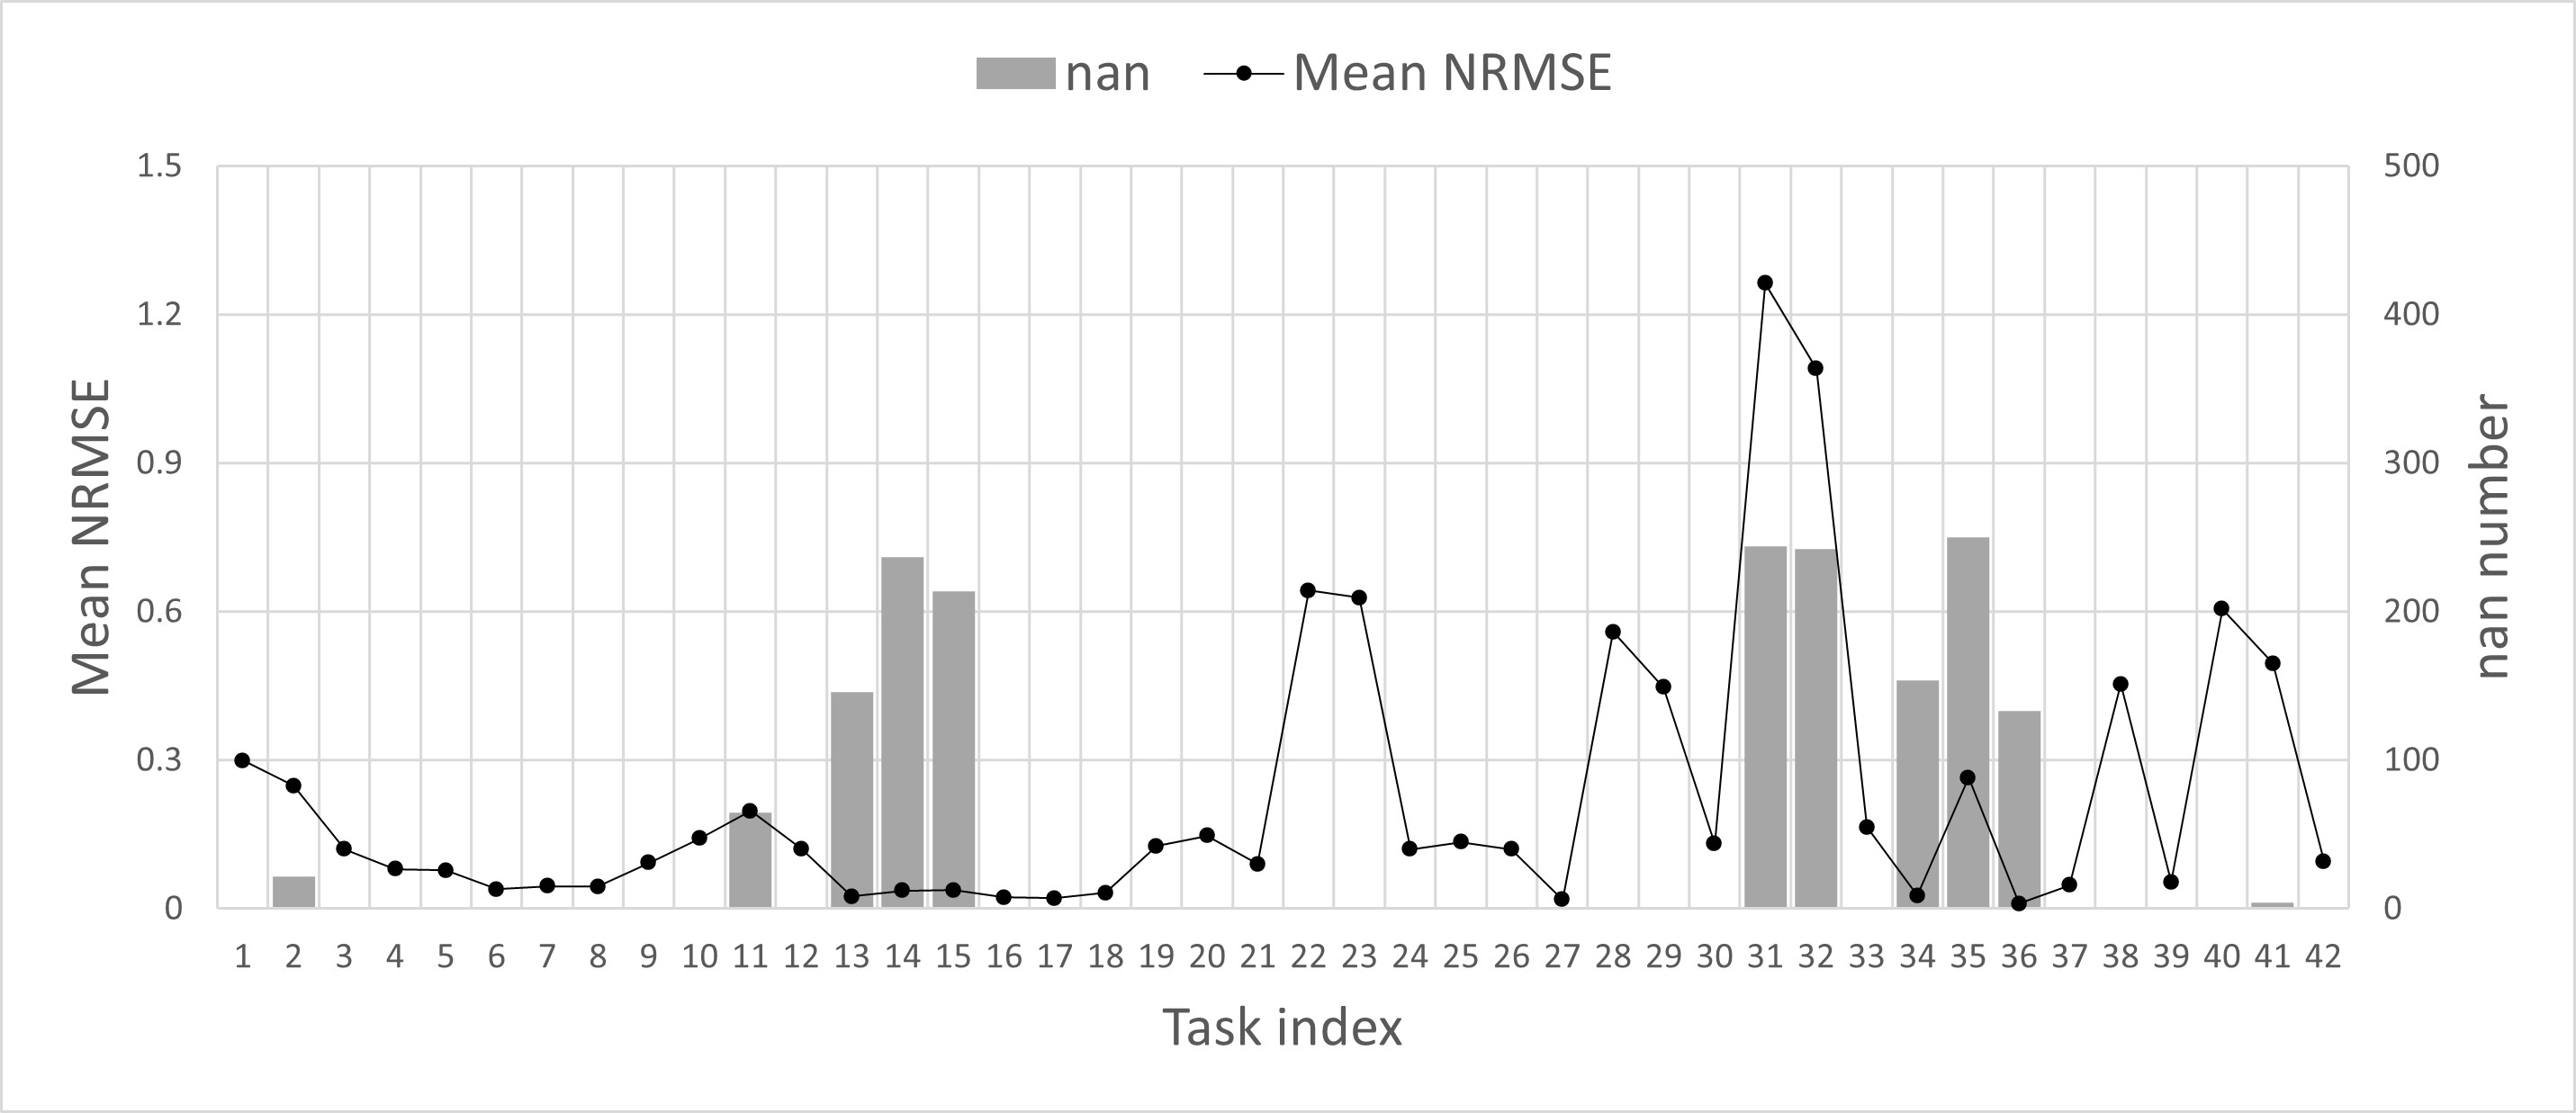
\includegraphics[width=14cm]{figure/ch4_fig_SAResults_BIClong.JPG}} \\
    \subfloat[]{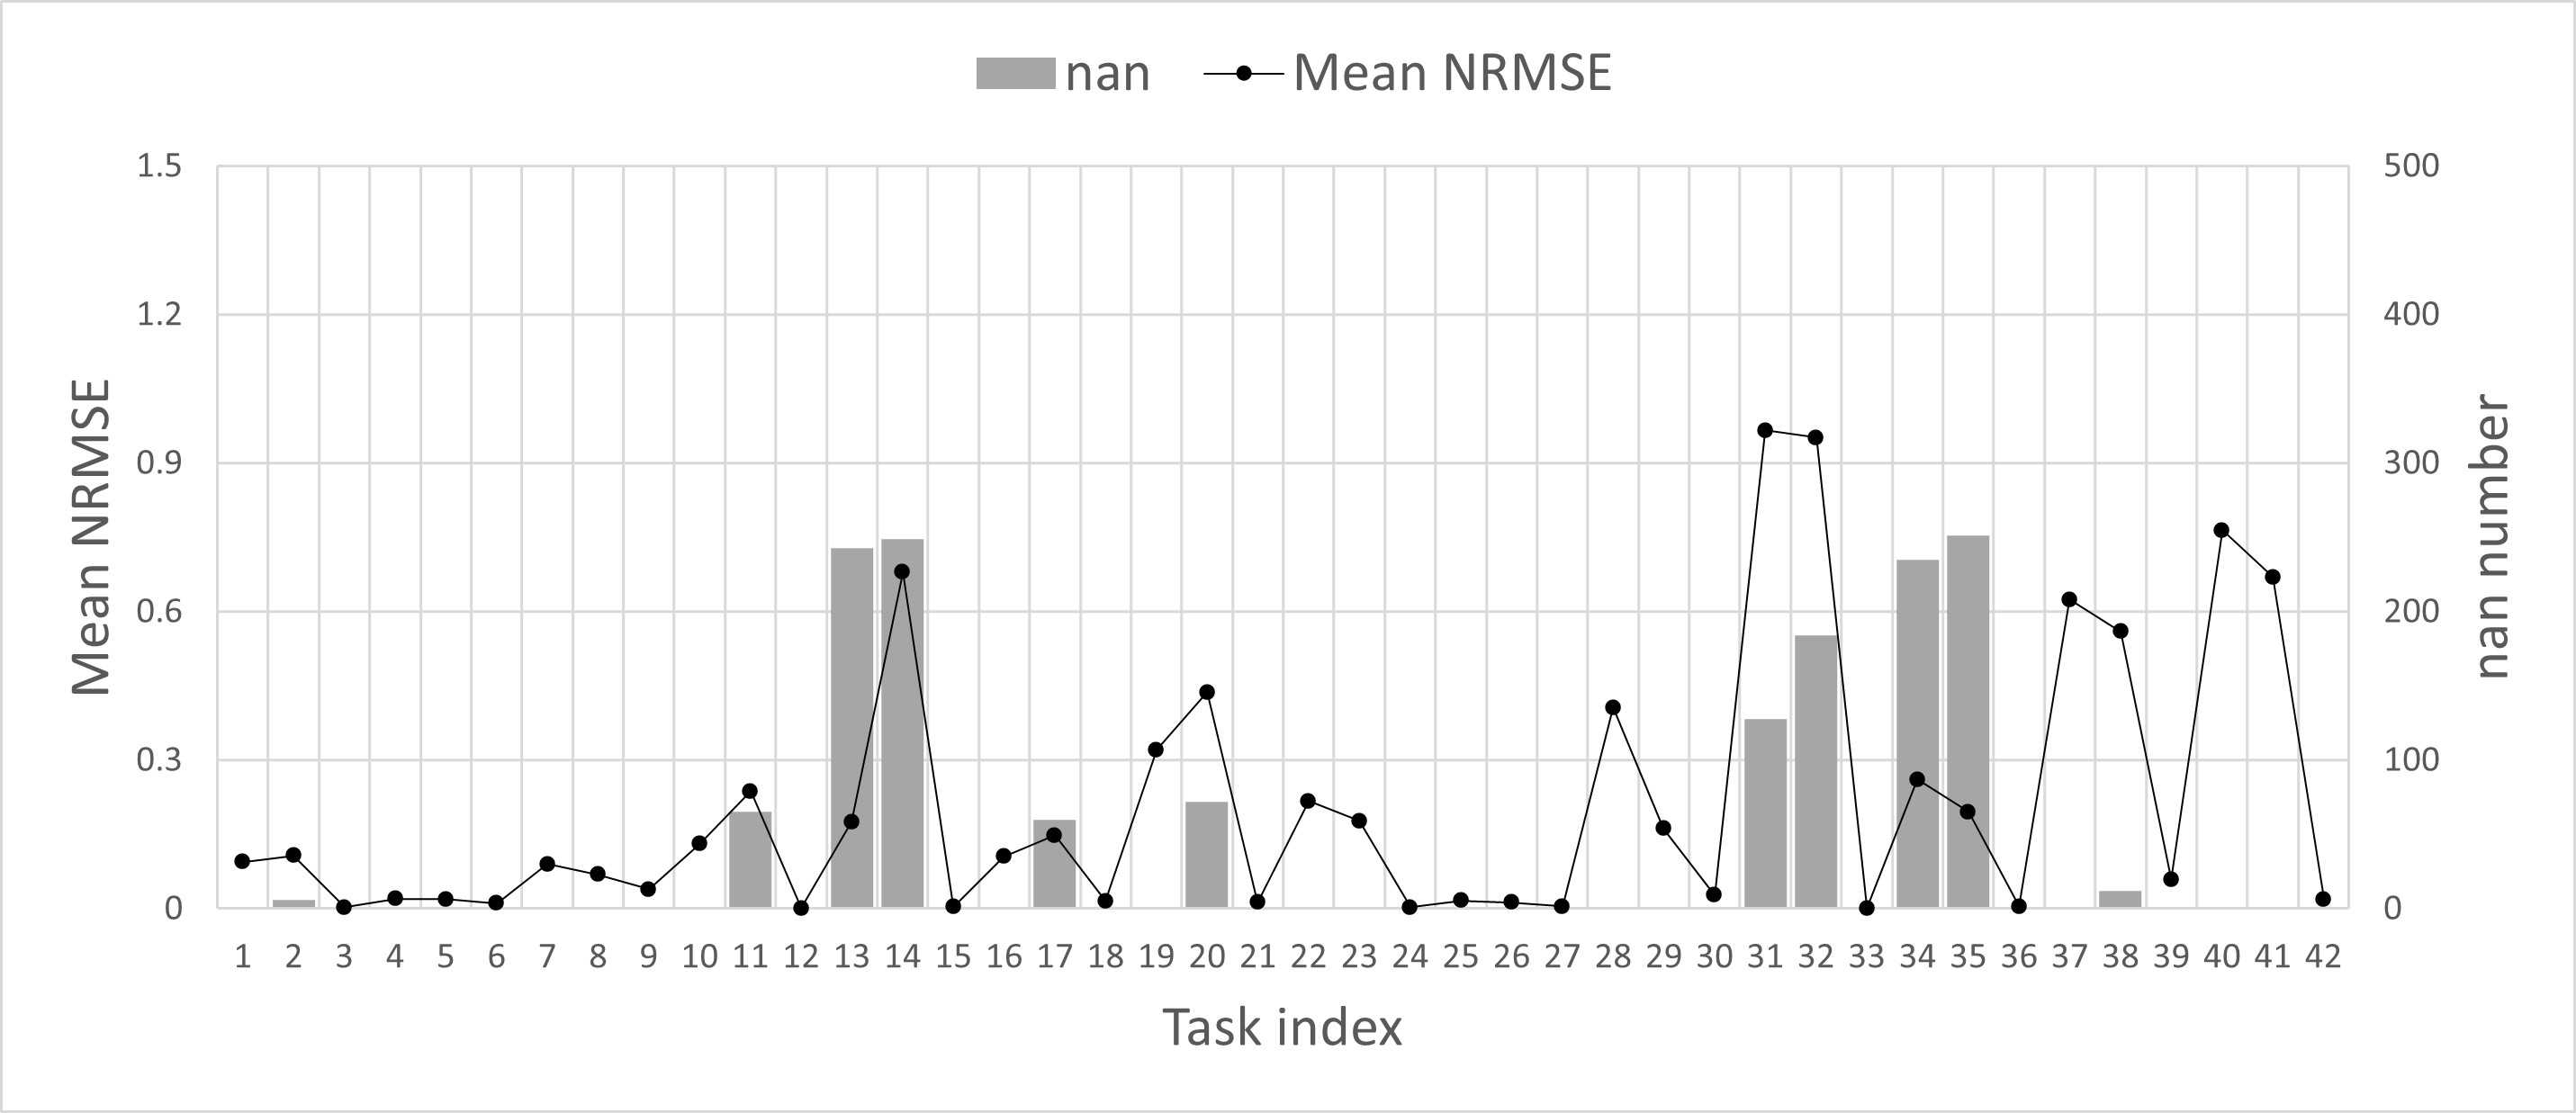
\includegraphics[width=14cm]{figure/ch4_fig_SAResults_BICshort.JPG}} 
    \caption[模擬案例之敏感度分析結果]{二頭肌 (a) 長頭與 (b) 短頭之敏感度分析結果。橫軸為任務編號;
                                     主座標軸 (左) 為全部樣本的 NRMSE 之平均值 (忽略 nan 值),即敏感度指標;
                                     副座標軸 (右) 為 NRMSE 為 nan 之樣本數量。}
    \label{ch4_fig_SAResults}
\end{figure}

% 敏感度高低差異
以圖 \ref{ch4_fig_SAExample} 的 Task 20 和 Task 17 比較作為範例說明,這兩個任務均為肘關節從 0 度伸展至 130 度,
唯獨差在 Task 20 的肩關節固定在 180 度,而 Task 17 則為 135 度,在相同的敏感度分析參數設置下擾動二頭肌長頭,
可明顯發現 Task 20 比 Task 17 的運動軌跡偏移還要大,代表二頭肌長頭對於 Task 20 有較高的敏感度,
其在模型的肌肉參數上有些許變動時,就會造成運動軌跡的大範圍偏離,而若是以敏感度低的任務作為執行任務,
則在估計過程容易把解附近的參數判定為答案,故敏感度分析的結果將對參數評估上有實質幫助。

\clearpage

\begin{figure}[!ht]
	\centering
	\subfloat[]{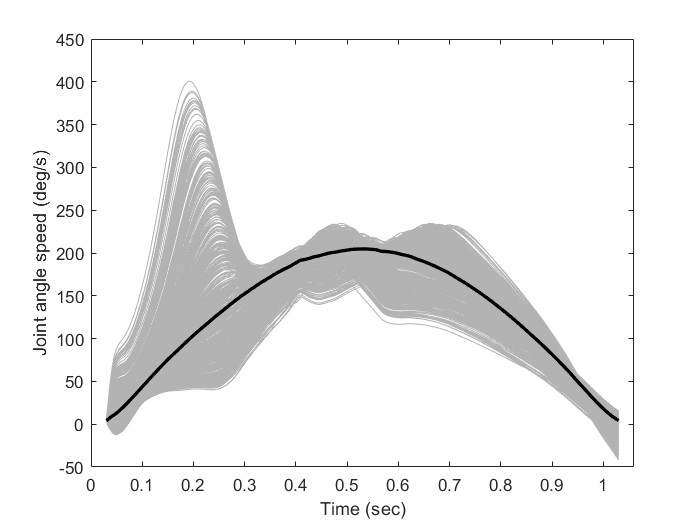
\includegraphics[width=7cm]{figure/ch4_fig_SAExample_20.JPG}}
    \subfloat[]{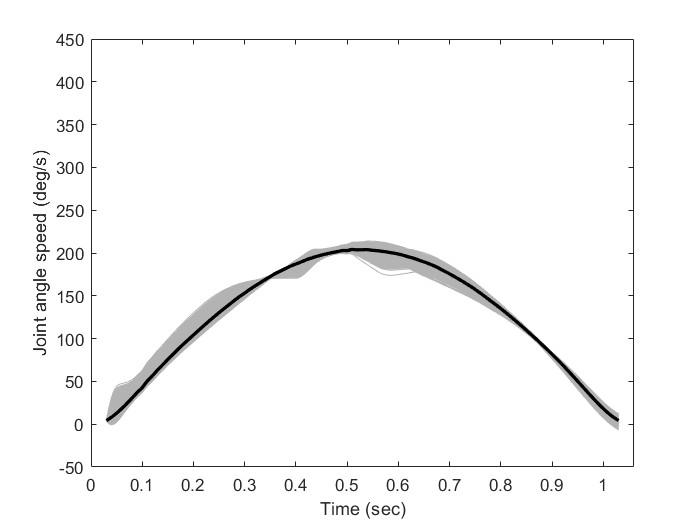
\includegraphics[width=7cm]{figure/ch4_fig_SAExample_17.JPG}} 
    \caption[呈現敏感度指標於運動軌跡偏移範例]{透過運動軌跡偏移來呈現 (a) Task 20 與 (b) Task 17 在二頭肌長頭的敏感度指標,
                                            其中 Task 20 與 Task 17 的敏感度指標分別為 0.1473 與 0.0208,                                      
                                            而圖中灰線代表擾動模型產生的軌跡,黑線則為目標軌跡。}
    \label{ch4_fig_SAExample}
\end{figure}

% ------------------------- 4.4 ------------------------- %
\section{肌肉參數最佳化與驗證}
% 兩個小節
本節將介紹參數評估的流程與設定,並依據上一節的任務挑選準則來挑選適當的任務,供後續的最佳化與模型驗證階段使用,
除了提供各個任務的敏感度分析結果外,亦會說明挑選的原因。

\subsection{最佳化與模型驗證}
% 程式流程圖
下方圖 \ref{ch4_flowchart_MKTP} 和 \ref{ch4_flowchart_Vali} 分別為執行多運動軌跡預測最佳化和驗證模型的程式流程圖,
在最佳化的參數設定上,上下界根據表 \ref{ch4_table_ModelDefaultParam} 來設定,
分別為 $100 \leq F^\mathrm{M}_\mathrm{O} \leq 1000$ 和 $0.05 \leq L^\mathrm{M}_\mathrm{O},L^\mathrm{T}_\mathrm{S} \leq 0.35$,
尋找初始值的容忍誤差則設定成 $f^{\mathbf{x}_0}_\mathrm{tol} \leq 0.05$,
而每個最佳化任務的預測誤差限制設定為 $E_\mathrm{tol} \leq 0.01$。

\begin{figure}[!ht]
	\centering
	\includegraphics[width=15cm]{figure/ch4_flowchart_MKTP.PNG}
    \caption[多運動軌跡預測最佳化之程式執行流程圖]{多運動軌跡預測最佳化之程式執行流程圖}
    \label{ch4_flowchart_MKTP}
\end{figure}

\begin{figure}[!ht]
	\centering
	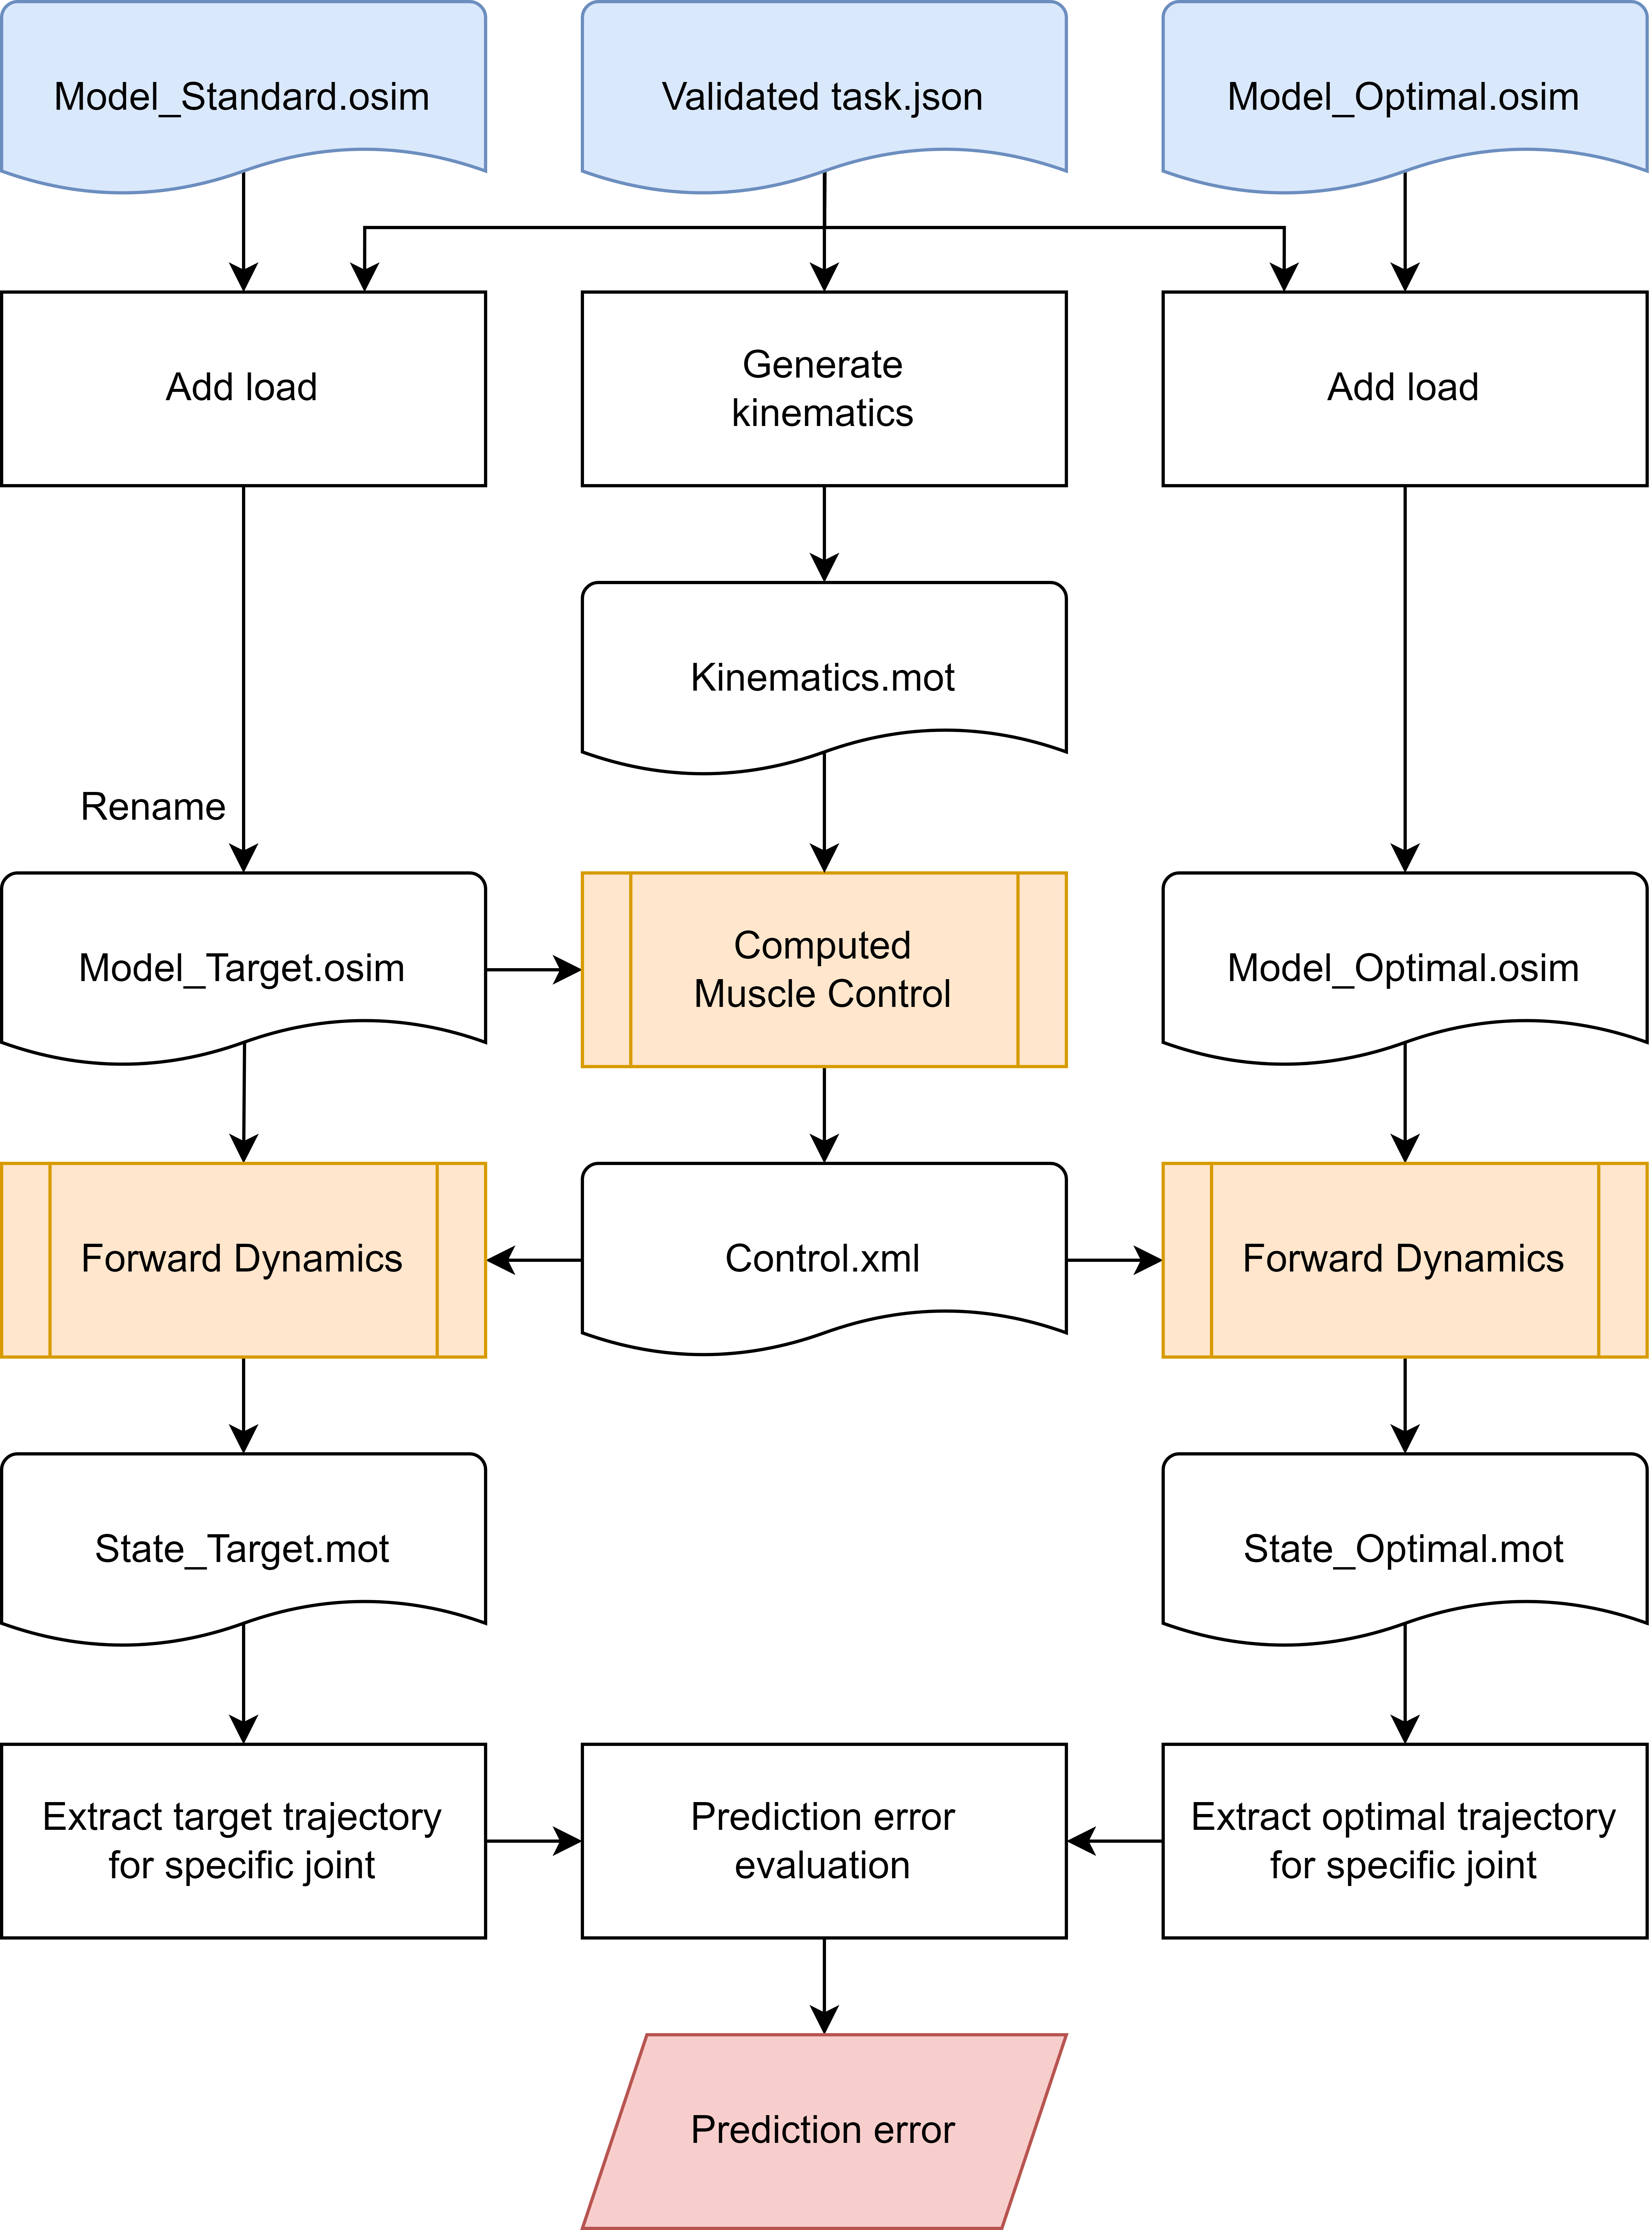
\includegraphics[width=11.5cm]{figure/ch4_flowchart_Vali.PNG}
    \caption[模型驗證之程式執行流程圖]{模型驗證之程式執行流程圖}
    \label{ch4_flowchart_Vali}
\end{figure}

\clearpage

\subsection{執行任務介紹}
% 挑選準則
以下將依據前一節所介紹的任務挑選準則與敏感度分析,針對欲評估的二頭肌肉群來挑選適當的任務,
並依序介紹各個任務的種類與性質。

\subsubsection{最佳化任務}
% Task * 2;挑選原因:健身;任務參數;敏感度分析參數;敏感度分析結果 * 2 muscle * 2 task
最佳化任務以常見的啞鈴彎舉動作來進行模擬,共挑選兩個任務來執行多運動軌跡預測最佳化,
分別為 Task 7 $(V_\mathrm{dir},\theta_\mathrm{sh},[\theta_1,\theta_2]) = (\text{flexion},0,[0,90])$
與 Task 8 $(V_\mathrm{dir},\theta_\mathrm{sh},[\theta_1,\theta_2]) = (\text{flexion},0,[0,130])$,
並將模型負重設定為 2.5 公斤來視為啞鈴。以下圖 \ref{ch4_fig_SAResults_Opt} 為這兩個任務與二頭肌群之敏感度分析結果,
在敏感度分析的參數設置上,樣本維持為 $N_\mathrm{sa} = 500$,而由於最佳化過程的上下界較為寬鬆,
且該任務為常見的健身動作,其目的只是為了藉由擾動來再次確認參數的更動是否對目標函數 ($E^\mathrm{mean}_\mathrm{NRMSE}$) 有影響,
故擾動值調整為 $\delta = 0.30$,這些擾動可假擬為參數在最佳化時的搜索過程。
圖 \ref{ch4_fig_SAResults_Opt} 中可看出擾動軌跡與目標軌跡皆有一定的差異程度,故用於執行最佳化是可行的。

\bigskip
\begin{figure}[!ht]
	\centering
	\subfloat[]{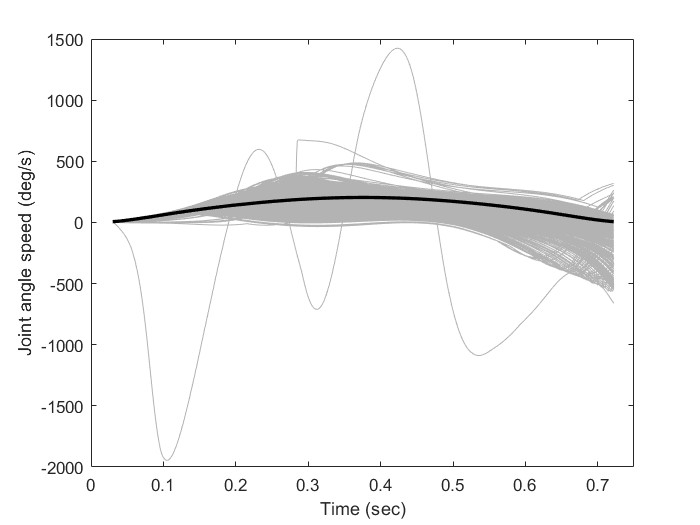
\includegraphics[width=6.99cm]{figure/ch4_fig_SAResults_OptLong_7.JPG}}
    \subfloat[]{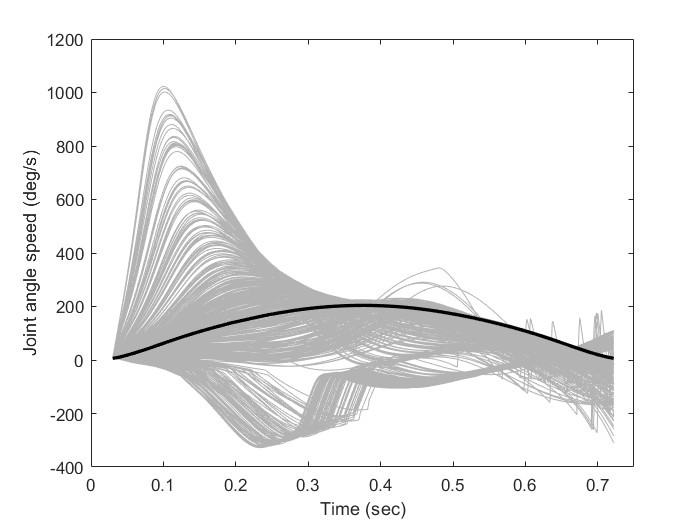
\includegraphics[width=6.99cm]{figure/ch4_fig_SAResults_OptShort_7.JPG}} \\  
    \subfloat[]{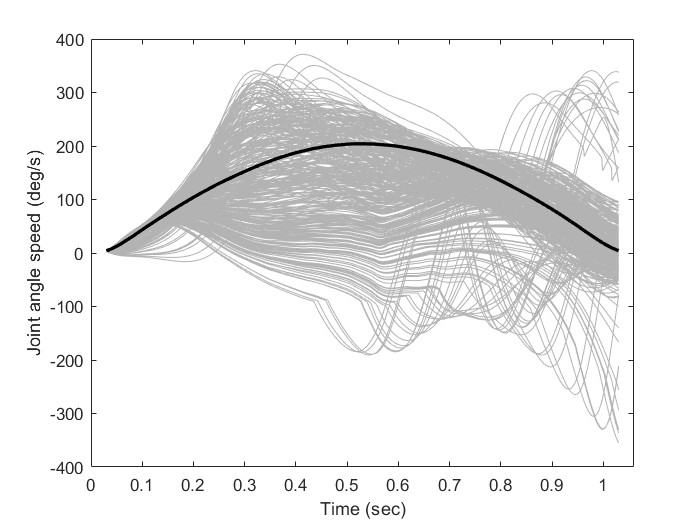
\includegraphics[width=6.99cm]{figure/ch4_fig_SAResults_OptLong_8.JPG}}
    \subfloat[]{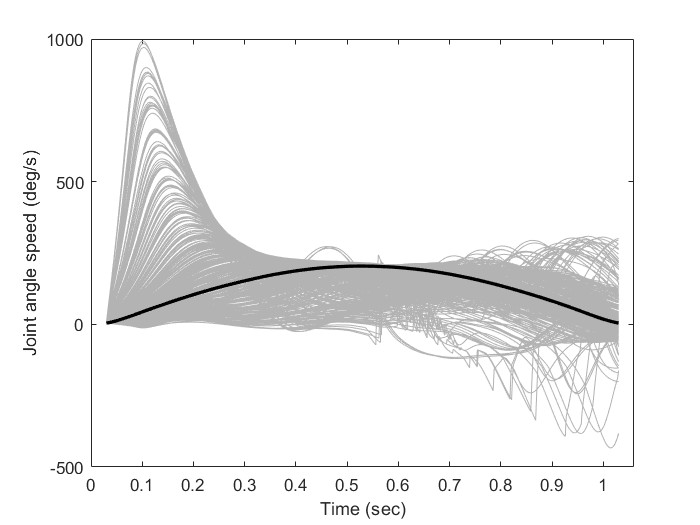
\includegraphics[width=6.99cm]{figure/ch4_fig_SAResults_OptShort_8.JPG}}
    \caption[最佳化任務之敏感度分析結果]{最佳化任務之敏感度分析結果:
                                       (a) Task 7 於二頭肌長頭之敏感度指標為 0.3919;
                                       (b) Task 7 於二頭肌短頭之敏感度指標為 0.5811;
                                       (c) Task 8 於二頭肌長頭之敏感度指標為 0.3421;
                                       (d) Task 8 於二頭肌短頭之敏感度指標為 0.4006。
                                       圖中灰線代表擾動模型產生的軌跡,黑線則為目標軌跡。}
    \label{ch4_fig_SAResults_Opt}
\end{figure}

\subsubsection{模型驗證任務}
% Task * 1;挑選原因:敏感度高;任務參數;敏感度分析參數;敏感度分析結果 * 2 muscle * 1 task
模型驗證的任務挑選則以高敏感度任務為優先,所挑選的任務為 Task 40 $(V_\mathrm{dir},\theta_\mathrm{sh},[\theta_1,\theta_2]) = (\text{extension},180,[0,90])$,
並同樣將負重設定為 2.5 公斤來模擬啞鈴。下方圖 \ref{ch4_fig_SAResults_Vali} 為驗證任務與二頭肌群之敏感度分析結果,
將樣本參數設置為 $N_\mathrm{sa} = 500$,擾動值則與先前的敏感度分析相同,設定為 $\delta = 0.05$,
藉由小範圍的擾動來檢視預設參數周圍的軌跡變動情形。最終敏感度分析結果顯示,即使是微小的參數變動,
其所產生的運動軌跡皆會有大幅的改變,該任務在驗證模型上將能有良好的鑑別作用。

\begin{figure}[!ht]
	\centering
	\subfloat[]{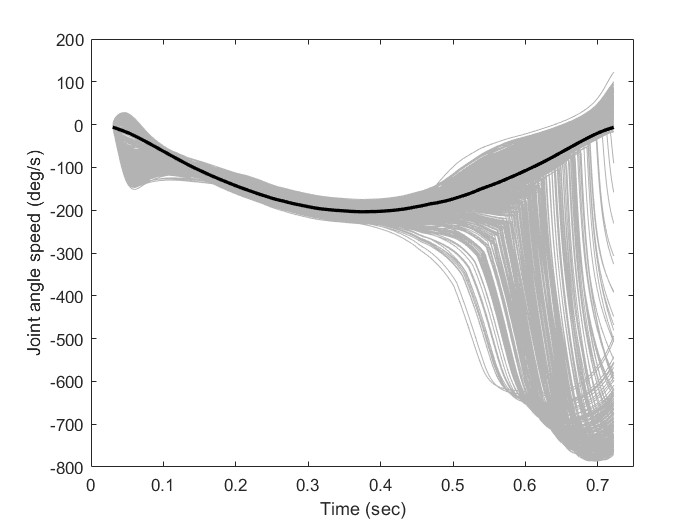
\includegraphics[width=6.99cm]{figure/ch4_fig_SAResults_ValiLong_40.JPG}}
    \subfloat[]{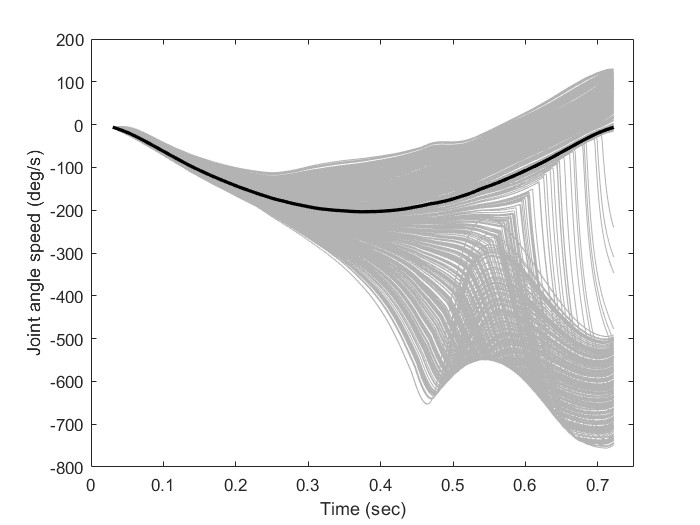
\includegraphics[width=6.99cm]{figure/ch4_fig_SAResults_ValiShort_40.JPG}} 
    \caption[模型驗證任務之敏感度分析結果]{模型驗證任務之敏感度分析結果:
                                         (a) Task 40 於二頭肌長頭之敏感度指標為 0.6050;
                                         (b) Task 40 於二頭肌短頭之敏感度指標為 0.7648。
                                         圖中灰線代表擾動模型產生的軌跡,黑線則為目標軌跡。}
    \label{ch4_fig_SAResults_Vali}
\end{figure}

% ------------------------- 4.5 ------------------------- %
\section{小結}
% 回顧;下章節再討論;從驗證結果證實方法有效
本章節將上肢肌肉骨骼模型套用在所提出的研究方法,介紹了許多模擬案例的細節,如負重功能的新增、運動軌跡公式、
任務種類等資訊,除此之外也先透過該模型來展示敏感度分析的結果,提供後續的最佳化與模型驗證的任務挑選,
最主要的目的是要完成上肢特定肌肉之參數評估。下個章節將依據第三章的研究方法、第四章的前置作業,
完整介紹參數評估案例,並針對評估結果進行探討。

\clearpage